\documentclass[a4paper,twoside,12pt]{article}
%% Language %%%%%%%%%%%%%%%%%%%%%%%%%%%%%%%%%%%%%%%%%%%%%%%%%
\usepackage[T1]{fontenc}
\usepackage[utf8]{inputenc}
\usepackage[english]{babel}
\usepackage[top=2.5cm, bottom=2.5cm, left=2.5cm, right=2.5cm]{geometry}
\usepackage{scrextend}
\addtokomafont{labelinglabel}{\sffamily}
\usepackage{lmodern} %Type1-font for non-english texts and characters
\usepackage{parskip}
\usepackage{enumitem}
\usepackage{parskip}
\setlength{\parskip}{12pt}

%% Packages for Graphics, Figures & Tables %%%%%%%%%%%%%%%%%%%%%%%%%%
\usepackage{graphicx} %%For loading graphic files
\usepackage{subcaption}
\usepackage{float}
\usepackage{booktabs} %% for top/midrule
\usepackage{textcomp}
\usepackage[table,xcdraw, dvipsnames]{xcolor}
\usepackage{tabularx}
\usepackage{longtable}
\usepackage{makecell}
\usepackage{pdflscape}
%bibliography
\usepackage[round]{natbib}
\bibliographystyle{abbrvnat}
\usepackage{hyperref}
\hypersetup{
    colorlinks=false,
    pdfborder={0 0 0} % Removes the border
}
\usepackage{geometry}
%% Math Packages %%%%%%%%%%%%%%%%%%%%%%%%%%%%%%%%%%%%%%%%%%%%
\usepackage{amsmath}
\usepackage{amsthm}
\usepackage{amsfonts}
%% Line Spacing %%%%%%%%%%%%%%%%%%%%%%%%%%%%%%%%%%%%%%%%%%%%%
\usepackage{setspace}
\onehalfspacing       %% 1,5-spacing
\usepackage{placeins}
\usepackage{lineno}
\linenumbers
\usepackage{titlesec}
\titlespacing{\section}{0pt}{*4}{*1.5} 
\titlespacing{\subsection}{20pt}{*4}{*1.5}
\titlespacing{\subsubsection}{40pt}{*4}{*1.5} 
\titlespacing{\paragraph}{60pt}{*4}{*1.5}
\titlespacing{\subparagraph}{80pt}{*4}{*1.5}
%%%%%%%%%%%%%%%%%%%%%%%%%%%%%%%%%%%%%%%%%%%%%%%%%%%%%%%%%%%%%
%% DOCUMENT
%%%%%%%%%%%%%%%%%%%%%%%%%%%%%%%%%%%%%%%%%%%%%%%%%%%%%%%%%%%%%
\begin{document}
 
\begingroup  
  \centering
\textbf{Long-term abundance time-series of the High Arctic terrestrial vertebrate community of Bylot Island, Nunavut}\\[1.5em]
 Louis Moisan\textsuperscript{1,2}, Azenor Bideault\textsuperscript{2,3}, Gilles Gauthier\textsuperscript{4}, Éliane Duchesne\textsuperscript{1}, 
 Dominique Fauteux\textsuperscript{5}, Dominique Berteaux\textsuperscript{1}, Pierre Legagneux\textsuperscript{3,6}, Marie-Christine Cadieux \textsuperscript{3} and Joël Bêty\textsuperscript{1}\\[1.5em]
\textbf{Author Affiliations}:\\
\textsuperscript{1} Chaire de Recherche du Canada en Biodiversité Nordique, Centre d’Études Nordiques, Centre de la Science de la Biodiversité du Québec, Département de Biologie, Chimie et Géographie, Université du Québec à Rimouski, Rimouski, QC, Canada\\
\textsuperscript{2} Chaire de Recherche du Canada en Écologie Intégrative, Centre d’Études Nordiques, Centre de la Science de la Biodiversité du Québec, Département de Biologie, Université de Sherbrooke, Sherbrooke, QC, Canada\\
\textsuperscript{3} Chaire de Recherche Sentinelle Nord sur l’Impact des Migrations Animales sur les Écosystèmes Nordiques, Centre d’Études Nordiques, Centre de la Science de la Biodiversité du Québec, Département de Biologie, Université Laval, Québec, QC, Canada\\
\textsuperscript{4} Centre d’Études Nordiques, Département de Biologie, Université Laval, Québec, QC, Canada\\
\textsuperscript{5} Centre d’Études Nordiques, Centre de Connaissance et d’Exploration de l’Arctique, Musée Canadien de la Nature, Ottawa, ON, Canada\\
\textsuperscript{6} Centre d’Études Biologiques de Chizé (CEBC-CNRS), Université de La Rochelle, France 
\\[1.5em]
\textbf{Corresponding Author}:\\
\textit{\href{mailto:louis.moisan.bio@gmail.com}{louis.moisan.bio@gmail.com}}\\
\textit{\href{mailto:joel_bety@uqar.ca}{joel{\textunderscore}bety@uqar.ca}}
\\[1.5em]
\textbf{Open Research statement}:\\
The data set is publicly available at \url{https://datadryad.org/XXXXXXX} and the raw data and codes used to extract the data set are publicly available at \url{https://zenodo.org/XXXXXXXXXX}.\\
\endgroup
\newpage

\subsection*{Introduction}
 The composition of ecological communities, defined as the abundance of each species within a given community, is fundamental for understanding patterns and processes in community ecology. Variations in community composition can help to detect spatial patterns linked to environmental variations \citep{kemp1990}, assess temporal trends of different groups of species after disturbances \citep{philippi1998, magurran2007}, and understand food web structures \citep{cohen2003}. Additionally, community composition is essential for modeling the dynamics of ecological communities. Dynamic community modelling allows addressing important issues and questions in ecology, such as: determining the relative strength of top-down versus bottom-up forces in communities \citep{krebs2003,legagneux2014}, assessing the ecological resilience of communities under climate change \citep{griffith2019} and evaluating the cascading effects of invasive species in food web \citep{david2017, goto2020}. Dynamic community modelling can also be applied to address practical challenges, including fishery management \citep{plaganyi2007} and the planning of protected areas \citep{okey2004, dahood2020}. 
 
Modeling food webs requires adjusting trophic flows based on the functional responses of species, which necessitates time series data on the abundance of all species within a community. However, determining the abundance of all species within a community is rarely achievable. Consequently, empirical community models often reduce taxonomic resolution by grouping species into large functional or taxonomic categories. Additionally, food webs consist of species with varying body sizes depending on their trophic level, with top-level species often being highly mobile and having large home ranges \citep{mccann2005}. Therefore, community models must use landscape-wide estimates of species abundance to accurately represent trophic fluxes. Due to these constraints, empirical datasets with high taxonomic resolution that cover entire communities at broad spatial and temporal scales are rare and often include incomplete or rough estimates.

The composition of ecological communities is influenced by various factors acting at different temporal and spatial scales, leading to noisy data and emphasizing the need for long-term data sets \citep{magurran2010, lindenmayer2012}. Species abundances are influenced by stochastic effects \citep{hubbell2001}, environmental changes (e.g., climate warming), and species interactions, contributing to data variability. For instance, the composition of a community could be driven simultaneously by intra-annual seasonal variations, multi-year cyclic variations (e.g., El Niño) and slow but directional long-term variations in the environment \citep{brown1990, snyder2006}. Therefore, long-term data series are required to untangle the relative effects of diverse abiotic and biotic factors on community composition \citep{magurran2010, lindenmayer2012}.

Arctic environments are highly valuable systems for studying community structure and dynamics due to their relatively low species richness \citep{payer2013, legagneux2014}. However, logistical challenges in the Arctic limit the number of long-term biodiversity monitoring programs. Hence, the small number of Arctic communities with long-term monitoring serve as highly valuable sites for holistic and empirical community studies. Datasets on terrestrial communities are notably scarce, and this scarcity extends to Arctic communities as well \citep{ims2013}.

Within terrestrial Arctic sites, the south plain of Bylot Island in the Canadian High Arctic (\textbf{Figure \ref{figure:food_web}}) hosts one of the longest and most intensive biodiversity monitoring programs \citep{gauthier2024a}. Monitoring on Bylot Island began in 1989 with a focus on the snow goose and it gradually expanded to other species over time. Currently, the program encompasses all significant vertebrate species in the community with continuous monitoring spanning more than a decade \citep{gauthier2024a}. Monitoring is also conducted at multiple spatial scales, including intensive and systematic observations conducted across a landscape spanning approximately 400 km\textsuperscript{2}. This approach allows the scaling of local density measurements to the landscape level when required and facilitates the estimation of abundance for less common and rare species.

Previous work based on the tundra community of Bylot Island  has already produced several influential papers \citep{gauthier2011, legagneux2012, legagneux2014,hutchison2020, duchesne2021, gauthier2024b}. These studies showed that tundra communities may experience stronger top-down regulation than bottom-up regulation \citep{legagneux2012, legagneux2014}. They also revealed a heterogeneous response of trophic levels to climate warming \citep{gauthier2013} and highlighted the effects of indirect trophic interactions on the occurrence of species across the landscape \citep{duchesne2021}. However, those earlier papers were built on data from relatively short time series, they were not always scaled at the landscape level, and some species or functional groups were lacking abundance estimates. With over a decade of additional community-wide monitoring compared to earlier studies, our goal is to synthesize and upscale the data collected on the Bylot Island community since the 1990s to the landscape level. This synthesis aims to provide readily accessible annual time series (or mean values in some cases) of abundance and biomass for all vertebrate species in a tundra landscape, covering approximately 400 km\textsuperscript{2}. 

\begin{figure}[H]
\centering
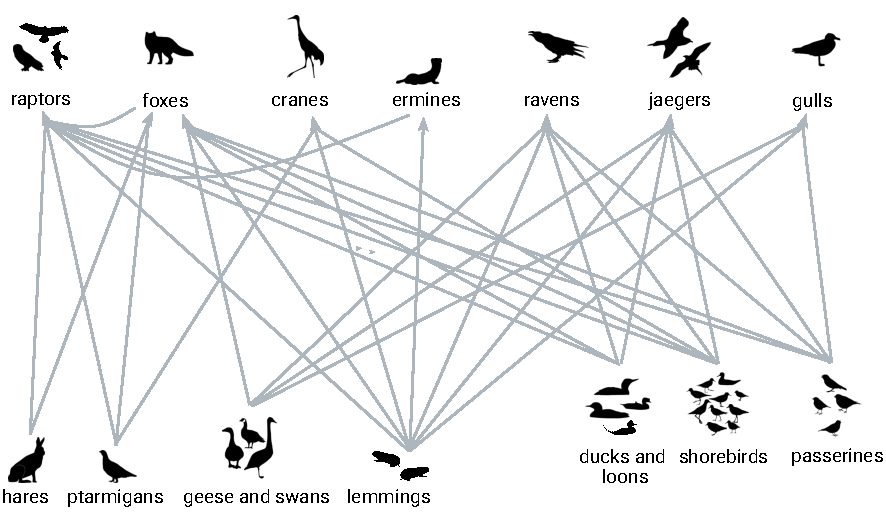
\includegraphics[width=0.75\linewidth]{figures/food_web.pdf} 
\caption{Synthetic vertebrate food web of the south plain of Bylot Island.}
\label{figure:food_web}
\end{figure}

\subsection*{Objective}
Our main objective is to provide readily accessible, long-term time series of annual abundances of all vertebrate species within the Arctic terrestrial community of Bylot Island during the breeding season (May to August). This includes both breeding and non-breeding individuals that stay in the study area for a significant period of time, and excludes non-breeding individuals that stop for only a few days during their migration. We focus on adults, except for lemmings for which we have not distinguished between juveniles and adults. Our focus extends to estimating abundances at the landscape scale, enabling the study of community and ecosystem dynamics, trophic interactions and the impacts of global changes on high-latitude environments. Additionally, we aim to provide the average body mass for each species in the community, enabling the conversion of abundances into biomasses.
\newpage
\section*{\textcolor{Blue}{Class I. Data Set Descriptors}}
    \section*{A. Data set identity} Long-term abundance time-series of the High Arctic terrestrial vertebrate community of Bylot Island, Nunavut
    \section*{B. Data set identification codes}
     \texttt{BYLOT-species\_taxonomy.csv}\\
     \texttt{BYLOT-species\_abundance.csv}\\
     \texttt{BYLOT-species\_body\_mass.csv}\\
     \texttt{BYLOT-interannual\_variation\_nest\_density.csv}\\
     
    \section*{C. Data set description}
                \subsection*{1. Originators}
                \textbf{Gilles Gauthier}, Centre d’Études Nordiques, Département de Biologie, Université Laval, Québec, QC, Canada\\
                \textbf{Joël Bêty},  Chaire de Recherche du Canada en Biodiversité Nordique, Centre d’Études Nordiques, Centre de la Science de la Biodiversité du Québec, Département de Biologie, Chimie et Géographie, Université du Québec à Rimouski, Rimouski, QC, Canada \\
                \textbf{Pierre Legagneux}, Chaire de Recherche Sentinelle Nord sur l’Impact des Migrations Animales sur les Écosystèmes Nordiques, Centre d’Études Nordiques, Centre de la Science de la Biodiversité du Québec, Centre d’Études Biologiques de Chizé (CEBC-CNRS) Département de Biologie, Université Laval, Québec, QC, Canada
                
                \subsection*{2. Abstract}
Arctic ecosystems present unique opportunities for community-wide monitoring, in part due to their relatively low species richness. However, conducting research in these remote environments poses significant logistical challenges, resulting in long-term monitoring being exceedingly rare. Here, we focus on the long-term, intensive ecological monitoring efforts conducted on the south plain of Bylot Island (almost 400 km\textsuperscript{2}, Nunavut, Canada), which has generated a remarkable dataset spanning up to 30 years, a rarity in tundra ecosystems. Our goal is to synthesize this dataset and upscale vertebrate abundance data at the landscape level, a prerequisite to conduct community-level analyses. We have standardized data obtained with different field methods to provide readily usable long-term time series of abundance for 35 vertebrate species (30 birds and 5 mammals) present in the study system. Monitoring data includes intensive capture-mark-recapture density estimates of lemmings on trapping grids, systematic or opportunistic nest monitoring conducted across the entire study area or within specific plots for all bird species, transects of vertebrate counts distributed throughout the study area, daily incidental observations of vertebrates and satellite tracking of fox movements. Annual abundance of species was estimated at the landscape level, accounting for spatial variations. Furthermore, we provide body masses for each species, derived from empirical onsite measurements for 18 species and from the literature for the remaining species. Body mass is essential to convert species abundance into biomass for studies of trophic fluxes and ecosystem processes. Our dataset provides a unique opportunity for holistic empirical studies of ecological communities, allowing a deeper understanding of community structure and dynamics. Considering that the study site is a pristine and protected area that has experienced minimal anthropogenic impact, it can also provide an ideal baseline for investigating the impacts of global changes on high-latitude terrestrial ecosystems.
   \section*{D. Key words/phrases}
 Bylot Island, Canadian Arctic, Arctic tundra, 1993-2023, long-term monitoring, biodiversity monitoring, community composition, species abundance, species density, species biomass, species body mass, food web
  \newpage
  
\section*{\textcolor{Blue}{Class II. Research origin descriptors}}
    \section*{A. Overall project description}
    \subsection*{1. Identity} Understanding the structure and dynamics of Arctic terrestrial communities
        \subsection*{2. Originators}   
        \textbf{Gilles Gauthier}, Centre d’études nordiques, Département de Biologie, Université Laval, Québec, QC, Canada\\
                \textbf{Joël Bêty},  Chaire de Recherche du Canada en Biodiversité Nordique, Centre d’Études Nordiques, Centre de la science de la biodiversité du Québec, Département de biologie, chimie et géographie, Université du Québec à Rimouski, Rimouski, QC, Canada \\
                \textbf{Pierre Legagneux}, Chaire de Recherche Sentinelle Nord sur l’impact des migrations animales sur les écosystèmes nordiques, Centre d’Études Nordiques, Centre de la science de la biodiversité du Québec, Centre d’Études Biologiques de Chizé (CEBC-CNRS) Département de Biologie, Université Laval, Québec, QC, Canada
        
        \subsection*{3. Period of study} 1989 - continuing
        
        \subsection*{4. Objectives}
       i) Understand the factors that shape the structure and drive the dynamics of Arctic terrestrial communities.\\
       ii) Predict the effects of current global environmental changes on the structure and dynamics of Arctic terrestrial communities.
       
     \subsection*{5. Abstract}
      Arctic terrestrial communities, characterized by relatively low species richness, offer unique opportunities for studying ecological patterns and dynamics in simplified systems. Despite their relative simplicity, these ecosystems feature complex species interactions, extreme seasonal environmental changes, and a significant proportion of migratory species, making it difficult to identify the key factors shaping their structure and dynamics. As global environmental changes accelerate, it is essential to understand the processes driving these communities to eventually predict future impacts on Arctic ecosystems. Our research combines long-term biodiversity monitoring, a community-wide approach, and food web modeling to address these challenges.
       
      \subsection*{6. Sources of funding}
Natural Sciences and Engineering Research Council of Canada, Fonds Québécois de Recherche Nature et Technologies, Centre d'études nordiques, Natural Resources Canada (Polar Continental Shelf Program), Network of Centers of Excellence Canada (ArcticNet), Canada First Research Excellence Fund (Sentinel North Program), Polar Knowledge Canada, Environment and Climate Change Canada, Canada Foundation for Innovation, Parks Canada Agency, International Polar Year program of the Government of Canada, Crown–Indigenous Relations and Northern Affairs Canada (Northern Contaminant Program), Duck Unlimited Canada, Kenneth M. Molson Foundation (Kenneth M. Molson Foundation’s donation for wildlife research, conservation, and habitat), Garfield Weston Foundation, First Air——Canadian North, Nunavut Wildlife Management Board, Université Laval, Université du Québec à Rimouski
\newpage
        
    \section*{B. Specific subproject description}
        \subsection*{1. Site description}
                        \subsubsection*{a. Site type}
  The study area (389 km\textsuperscript{2}) represents a relatively productive tundra ecosystem in the eastern Canadian High-Arctic. An important biological characteristic of the area is the presence of a large snow goose (scientific names of most vertebrate species can be found in \textbf{Table \ref{table:table_species_name_strategy}}) colony of around 25 000 breeding pairs \citep{reed2002} spanning approximately 70 km\textsuperscript{2}. The vertebrate community within the study area comprises 30 bird species, with 29 of them being migratory or partially migratory, along with 5 mammal species (\textbf{Table \ref{table:table_species_name_strategy}}; \citet{moisan2023, gauthier2024a}). The study area experiences significant temporal fluctuations in the population of small mammals (lemmings), which in turn impact the occurrence and abundance of their avian and mammalian predators such as snowy owls, rough-legged hawks, long-tailed jaegers, ermines and Arctic foxes \citep{legagneux2012, duchesne2021}. We exclude occasional visitors, namely: i) species lacking confirmed breeding occurrences on the study site, ii) species observed solely within a single year, and iii) species primarily breeding and foraging in nearby marine or coastal habitats \citep{moisan2023}. The case of the red fox (\textit{Vulpes vulpes}) was ambiguous. While the presence of breeding pairs has been confirmed in the study area \citep{lai2022}, the extent of population establishment remains unclear and sightings are rare. Therefore, we decided to exclude this species.
                        % latex table generated in R 4.4.1 by xtable 1.8-4 package
% Mon Oct  7 10:12:12 2024
\begin{table}[ht]
\centering
\caption{Species of the vertebrate community of Bylot Island and their corresponding migratory status (i.e., resident, partial migrant or migrant).} 
\label{table:table_species_name_strategy}
\begingroup\fontsize{10pt}{10pt}\selectfont
\begin{tabularx}{0.97\textwidth}{llll}
  \hline
{\textbf{Functional group}} & {\textbf{Scientific name}} & {\textbf{English name}} & {\textbf{Migratory status}} \\ 
  \hline
Ducks and loons  & {\emph{ Gavia pacifica}} & Pacific loon & migrant \\ 
  Ducks and loons  & {\emph{ Gavia stellata}} & Red-throated loon & migrant \\ 
  Ducks and loons  & {\emph{ Somateria spectabilis}} & King eider & migrant \\ 
  Ducks and loons  & {\emph{ Clangula hyemalis}} & Long-tailed duck & migrant \\ 
  Geese and swans  & {\emph{ Branta hutchinsii}} & Cackling goose & migrant \\ 
  Geese and swans  & {\emph{ Anser caerulescens}} & Snow goose & migrant \\ 
  Geese and swans  & {\emph{ Cygnus columbianus}} & Tundra swan & migrant \\ 
  Raptors  & {\emph{ Buteo lagopus}} & Rough-legged hawk & migrant \\ 
  Raptors  & {\emph{ Falco peregrinus}} & Peregrine falcon & migrant \\ 
  Raptors  & {\emph{ Bubo scandiacus}} & Snowy owl & migrant \\ 
  Ptarmigans  & {\emph{ Lagopus muta}} & Rock ptarmigan & resident \\ 
  Cranes  & {\emph{ Antigone canadensis}} & Sandhill crane & migrant \\ 
  Shorebirds  & {\emph{ Pluvialis dominica}} & American golden-plover & migrant \\ 
  Shorebirds  & {\emph{ Pluvialis squatarola}} & Black-bellied plover & migrant \\ 
  Shorebirds  & {\emph{ Charadrius hiaticula}} & Common-ringed plover & migrant \\ 
  Shorebirds  & {\emph{ Arenaria interpres}} & Ruddy turnstone & migrant \\ 
  Shorebirds  & {\emph{ Calidris canutus}} & Red knot & migrant \\ 
  Shorebirds  & {\emph{ Calidris melanotos}} & Pectoral sandpiper & migrant \\ 
  Shorebirds  & {\emph{ Calidris bairdii}} & Baird's sandpiper & migrant \\ 
  Shorebirds  & {\emph{ Calidris fuscicollis}} & White-rumped sandpiper & migrant \\ 
  Shorebirds  & {\emph{ Calidris subruficollis}} & Buff-breasted sandpiper & migrant \\ 
  Shorebirds  & {\emph{ Phalaropus fulicarius}} & Red phalarope & migrant \\ 
  Gulls  & {\emph{ Larus hyperboreus}} & Glaucous gull & migrant \\ 
  Jaegers  & {\emph{ Stercorarius longicaudus}} & Long-tailed jaeger & migrant \\ 
  Jaegers  & {\emph{ Stercorarius parasiticus}} & Parasitic jaeger & migrant \\ 
  Ravens  & {\emph{ Corvus corax}} & Common raven & partial migrant \\ 
  Passerines & {\emph{ Eremophila alpestris}} & Horned lark & migrant \\ 
  Passerines & {\emph{ Anthus rubescens}} & American pipit & migrant \\ 
  Passerines & {\emph{ Calcarius lapponicus}} & Lapland longspur & migrant \\ 
  Passerines & {\emph{ Plectrophenax nivalis}} & Snow bunting & migrant \\ 
  Lemmings  & {\emph{ Lemmus trimucronatus}} & Nearctic brown lemming & resident \\ 
  Lemmings  & {\emph{ Dicrostonyx groenlandicus}} & Nearctic collared lemming & resident \\ 
  Hares  & {\emph{ Lepus arcticus}} & Arctic hare & resident \\ 
  Ermines  & {\emph{ Mustela richardsonii}} & American ermine & resident \\ 
  Foxes  & {\emph{ Vulpes lagopus}} & Arctic fox & partial migrant \\ 
   \hline
\end{tabularx}
\endgroup
\end{table}

%label-> table:table_species_name_strategy
\newpage
                \subsubsection*{b. Geography} Our 389 km\textsuperscript{2} study area is located on the southern plain of Bylot Island, Nunavut, Canada (72.889 N, -79.906 W; \textbf{Figure \ref{figure:zones}}).
                \subsubsection*{c. Habitat}  The study area comprises a combination of mesic tundra mainly on hills (64 \%), upland plateaus of sedimentary rock with drier/rockier habitat at higher elevation (20 \%), low-lying wetlands interspersed with ponds (10 \%) and larger bodies of water such as lakes and rivers (6 \%).
                \subsubsection*{d. Geology} See \citet{klassen1993} for a detailed description of the geology of the study area.
                \subsubsection*{e. Hydrology} Wetlands were delineated by photo-interpretation of high-resolution satellite images (30 cm; Louis-Pierre Ouellet, unpublished data), whereas lakes were delineated with aerial photos and rivers with google satellite images, resulting in a coarser delineation.
                \subsubsection*{f. Site history} See \citet{gauthier2024a, gauthier2024b}  for a complete and detailed history of the site.
                \subsubsection*{g. Climate} The mean annual air temperature since 1995 is -14.4°C, with mean seasonal temperature of 4.7°C in summer (June to August), -11°C in fall (September to November), -32.4°C in winter (December to February) and -19.4°C in spring (March to May; \citet{bylotclimate}). The climate of the southern plain of Bylot Island is generally milder than that of the surrounding latitudes, as the plain present a southern exposure and the mountains to the north protect the plain from cold northerly winds \citep{gauthier2024a}. In summer, the study area received on average 77.5 mm of precipitation \citep{bylotclimate}. Additionnally, 102 days are frost-free annually on average  \citep{bylotclimate} and the study area typically remains free of snow from mid-June to late September \citep{gauthier2013}.
\newpage
       
        \subsection*{2. Experimental or sampling design}
                        \subsubsection*{a. Permanent plots}
The study area is divided into 9 zones based on the sampling method and the level of field effort applied in each zone (\textbf{Figure \ref{figure:zones}}). Long-term monitoring of the community began in the 1990s in the Qarlikturvik valley \citep{gauthier2013, gauthier2024a}, which represents the zone of the study area with the highest annual sampling effort. Within the Qarlikturvik valley, the sampling is concentrated on the southern side of the glacial river (\textbf{Figure \ref{figure:qarlikturvik_valley}}), where the main research infrastructure is located. Another zone with extensive sampling efforts is Camp 2, located at the core of the snow goose colony, where the primary focus is to monitor snow goose nests. However, nests of many other avian species are also monitored within and around the colony in this zone. Camp 3, Pointe Dufour, Goose Point, and Malaview are zones where intensive sampling efforts are conducted annually, albeit for a relatively brief period (approximately one week) during the breeding season of most species \citep{gauthier2024a}. The upland zones in the study area (defined as areas approximately 300 meters above sea level or more) are the Black Plateau, Southern Plateau, and Camp 3 Plateau. These zones are primarily visited to assess raptor nesting activity \citep{beardsell2016}. The zone between the Qarlikturvik valley and Camp 3 received very little sampling effort and is therefore excluded from the study area.
\begin{figure}
\centering
  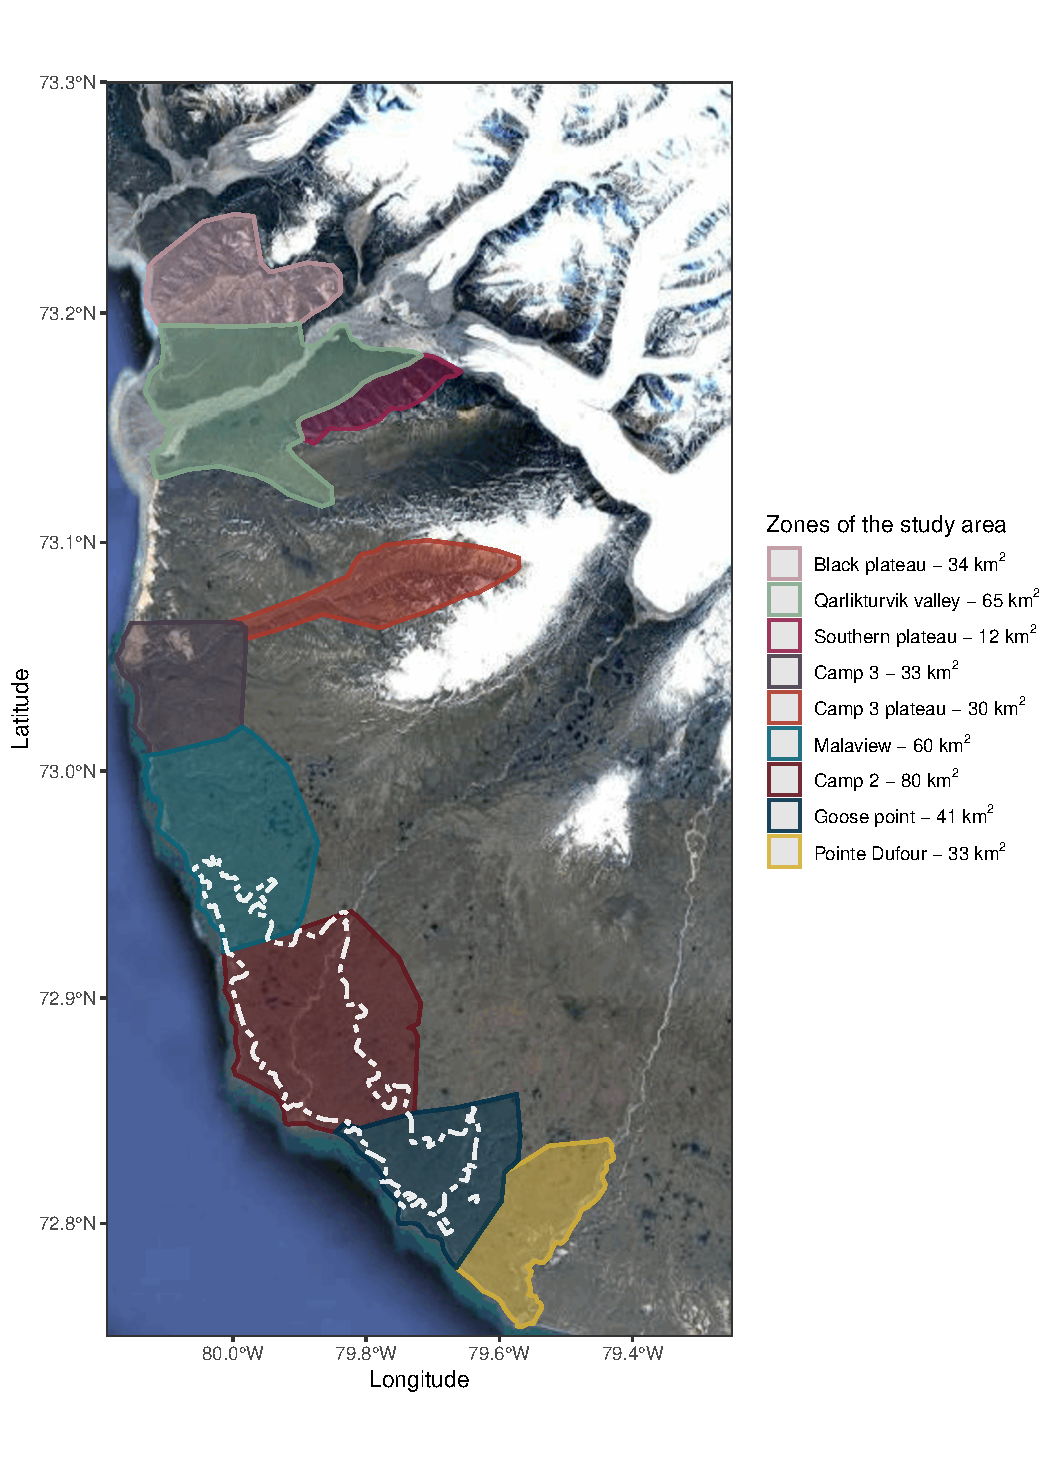
\includegraphics[width=0.8\textwidth, angle=0]{figures/zones_study_area.pdf}
   \caption{Map of the different zones (colored polygons) of the 389 km\textsuperscript{2} study area located on the south plain of Bylot Island, Nunavut Canada. The perimeter of the snow goose colony is delineated by white dashes; we highlighted the perimeter in 2017 since it represents the average colony area (74 km\textsuperscript{2}).}
  \label{figure:zones}
\end{figure}
\begin{figure}
\centering
  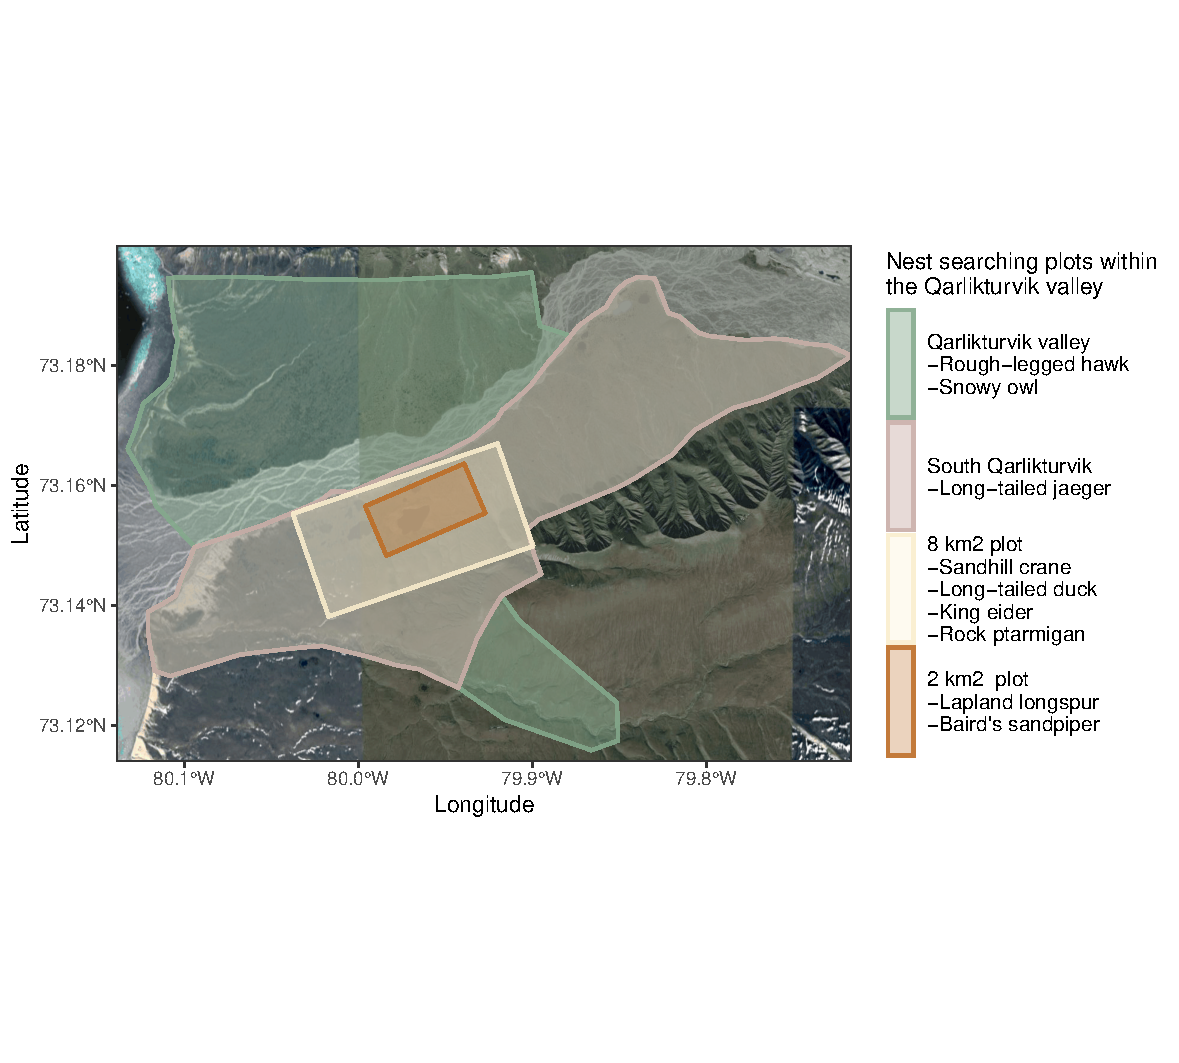
\includegraphics[width=0.8\textwidth, angle=0]{figures/qarlikturvik_valley.pdf}
  \vspace{-70pt} % Reduce space between figure and caption
  \caption{Intensive nests searching plots within the Qarlikturvik valley.}
 \label{figure:qarlikturvik_valley}
\end{figure}
\newpage
                \subsubsection*{b. Avian nest monitoring}
Avian nest monitoring was not conducted in 2020 and 2021 due to logistical constraints imposed by the COVID-19 pandemic. Systematic nest monitoring refers here to a systematic sampling approach aimed at documenting all nests within a specified area. Monitoring is considered opportunistic when there is a chance that some nests might not have been detected within a specific area. Nest densities derived from nest sampling could be underestimated due to early nest failure (i.e., failure that happened before our sampling period).
% latex table generated in R 4.4.1 by xtable 1.8-4 package
% Thu Oct 10 16:07:48 2024
\begin{table}[ht]
\centering
\caption{Summary of vertebrate species monitoring in the Bylot Island study area. In this paper, we excluded certain years for specific species due to reduced sampling efforts. As a result, duration of times series presented here may differ slightly from those in Gauthier et al. (2024b).} 
\label{table:table_species_year_monitoring}
\begingroup\fontsize{8pt}{10pt}\selectfont
\begin{tabularx}{\textwidth}{lllll}
  \hline
{\textbf{Species}} & {\textbf{Zone}} & {\textbf{Years}} & {\textbf{Number of years}} & {\textbf{Monitoring}} \\ 
  \hline
Pacific loon & Qarlikturvik valley & 2004-2019, 2022 & (17) & systematic \\ 
  Pacific loon & Whole study area & 2017-2019, 2022 & (4) & systematic \\ 
  Red-throated loon & Qarlikturvik valley & 2004-2019, 2022 & (17) & systematic \\ 
  Red-throated loon & Whole study area & 2017-2019, 2022 & (4) & systematic \\ 
  King eider & Qarlikturvik (8 km2 plot) & 2005-2019, 2022 & (16) & opportunistic \\ 
  Long-tailed duck & Qarlikturvik (8 km2 plot) & 2005-2019, 2022 & (16) & opportunistic \\ 
  Cackling goose & Qarlikturvik valley & 2004-2019, 2022-2023 & (18) & systematic \\ 
  Cackling goose & Whole study area & 2017-2019, 2022-2023 & (5) & systematic \\ 
  Snow goose & Camp 2 & 1999-2019, 2023 & (22) & systematic \\ 
  Tundra swan & Qarlikturvik valley & 2004-2019, 2022 & (17) & systematic \\ 
  Tundra swan & Whole study area & 2017-2019, 2022 & (4) & systematic \\ 
  Rough-legged hawk & Qarlikt., Black \& South plat. & 2007-2019, 2022 & (15) & systematic \\ 
  Rough-legged hawk & Whole study area & 2013-2019, 2022 & (8) & systematic \\ 
  Peregrine falcon & Qarlikt., Black \& South plat. & 2007-2019, 2022 & (15) & systematic \\ 
  Peregrine falcon & Whole study area & 2013-2019, 2022  & (8) & systematic \\ 
  Snowy owl & Qarlikt., Black \& South plat. & 1996-2019, 2023 & (25) & systematic \\ 
  Snowy owl & Whole study area & 2012-2019, 2022-2023 & (10) & systematic \\ 
  Rock ptarmigan & Qarlikturvik (8 km2 plot) & 2005-2019, 2022 & (16) & opportunistic \\ 
  Sandhill crane & Qarlikturvik (8 km2 plot) & 2005-2019, 2022 & (16) & opportunistic \\ 
  Common-ringed plover & Whole study area & 2015-2017 & (3) & systematic \\ 
  Baird's sandpiper & Qarlikturvik (2 km2 plot) & 2005-2019, 2022-2023 & (17) & systematic \\ 
  Glaucous gull & Qarlikturvik valley & 2004-2019, 2022 & (17) & systematic \\ 
  Glaucous gull & Whole study area & 2017-2019, 2022 & (4) & systematic \\ 
  Long-tailed jaeger & South Qarlikturvik valley & 2004-2019, 2022 & (17) & systematic \\ 
  Parasitic jaeger & South Qarlikturvik valley & 2004-2019, 2022 & (17) & systematic \\ 
  Parasitic jaeger & Whole study area & 2009-2019, 2022 & (12) & opportunistic \\ 
  Common raven & Whole study area & 2013-2019, 2022 & (8) & systematic \\ 
  Lapland longspur & Qarlikturvik (2 km2 plot) & 2005-2019, 2022-2023 & (17) & systematic \\ 
  Nearctic brown lemming & Qarlikturvik (trapping grids) & 1995-2019, 2021-2022 & (27) & systematic \\ 
  Nearctic collared lemming & Qarlikturvik (trapping grids) & 1995-2019, 2021-2022 & (27) & systematic \\ 
  American ermine & Whole study area & 1993-2019 & (27) & opportunistic \\ 
  Arctic fox & Whole study area & 2008-2016 & (9) & systematic \\ 
   \hline
\end{tabularx}
\endgroup
\end{table}

%label-> table:table_species_year_monitoring
        \begin{enumerate}[label=\roman*]
        \item[] \textit{\textbf{Pacific loon, red-throated loon, cackling goose, tundra swan and glaucous gull}}\\
        Since 2004, systematic searches of wetland areas have been conducted on the southern side of the glacial river in the Qarlikturvik valley, and since 2017, in other zones of the study area. This sampling aimed to find all nests of the cackling goose and the glaucous gull. Nest locations of other large wetland-nesting species, including the tundra swan, the red-throated loon and the Pacific loon, were also noted, as these species nest in the same habitat \citep{duchesne2021,gauthier2024a}. Each year, all known or potential nesting sites were revisited. Observers detected nests by walking and scanning around ponds and lakeshores to identify any active nesting sites. These large species can be seen from a relatively long distance sitting on the nest or when flushing from the nest. Most of them (geese, swans and gulls) can also reveal their presence with alarm calls or nest defense displays. We are confident that nest detection probability was high for these species given the open landscape.
        
        \item[] \textit{\textbf{Snow goose}}\\
        Snow geese nest in a large colony in the study area (\textbf{Figure \ref{figure:zones}}), but also in small aggregations distributed on the island, especially in years when snowy owls are nesting \citep{lepage1996,reed2002}. Since 1994, goose nests were systematically monitored on a 0.24 km\textsuperscript{2} wetland at the center of the colony. Since 1999, nests were also systematically monitored on a variable number of plots, measuring 0.01 km\textsuperscript{2} in wetland habitat and 0.04 km\textsuperscript{2} in mesic habitat, randomly distributed throughout the goose colony \citep{gauthier2020goose}. The total area covered by the randomly distributed plots averaged 0.79 \textpm{0.37} km\textsuperscript{2} per year. From 2010 onwards, except in 2020 and 2021, we opportunistically traced sections of the approximate boundary of the goose colony using a GPS receiver aboard a helicopter, taking advantage of regular flights across the study area whenever the flight path passed over the colony border \citep{duchesne2021}.
        
        \item[] \textit{\textbf{Rough-legged hawk, peregrine falcon and common raven}}\\
        Peregrine falcons, rough-legged hawks and common ravens nest on cliffs, near ravines, and on large rocky outcrops and tend to reuse the same nesting sites from one year to the next \citep{beardsell2016}. Systematic monitoring of every known or potential nesting site has been carried out in the Qarlikturvik valley, Black plateau and Southern plateau since 2007 and throughout the study area since 2013 \citep{beardsell2016, gauthier2020avianpred}. Observers walked along ridges and scanned surrounding areas from vantage points to detect nesting birds. These large species can be seen from a relatively long distance sitting on the nest or when flushing from the nest. They can also reveal their presence with alarm calls or nest defense displays. We are confident that nest detection probability was high for these species. Each year the observers use slightly different paths to sample the areas, but locate the nests in the same positions, which supports a high probability of detection for these species. Most nesting sites were located in the upland zones of the study area, which include the Black Plateau, Southern Plateau and Camp 3 Plateau.
        
        \item[] \textit{\textbf{Snowy owl}} \\
        Snowy owls predominantly nest in habitats similar to other raptors, favoring ridges in mountainous or hilly regions, although they can occasionally be found nesting on mounds in lowland areas \citep{seyer2020}. Since 1996, searches for snowy owl nests have been conducted concurrently with searches for other raptor nests in the Black and Southern plateaus, as well as during searches for jaeger nests on the southern side of the glacial river in the Qarlikturvik Valley. Additionally, since 2012, nests have been recorded across the entire study area by scanning the landscape from hills and ridges during the nesting period \citep{duchesne2021}. Given that snowy owls nest on elevated mounds, exhibit contrasting colors with the landscape, emit alarm calls, and display defensive behaviors, active nesting sites have a high probability of detection.
        
        \item[] \textit{\textbf{Long-tailed jaeger and parasitic jaeger}} \\
        Since 2004, observers have walked parallel transects spaced 400 meters apart, covering the entire southern side of the glacial river in the Qarlikturvik Valley (33 km\textsuperscript{2}; \textbf{Figure \ref{figure:qarlikturvik_valley}}), during the nesting period. The aim of those transects was to record nests of long-tailed jaegers, parasitic jaegers, and sandhill cranes. Observers listened for alarm calls to detect territorial birds, and then located nests by observing the birds returning to their nests from elevated vantage points. We consider the sampling to be systematic for long-tailed and parasitic jaeger, since those species tend to leave their nest relatively far from the observer to perform mobbing behavior, and thus increasing their detection probability. We do not consider the sampling to be systematic for sandhill cranes as they only display defensive behaviors near their nests at relatively short distances (see opportunistic nest monitoring below).
        
        \item[] \textit{\textbf{Common-ringed plover}} \\
        Between 2015 and 2019, observers conducted surveys of the primary nesting areas of the common-ringed plover. The survey involved walking in stony and sandy shores and gravel bars with scarce vegetation along rivers. Nests were found by detecting individuals exhibiting reproductive behaviors, such as incubation, alarm calls, or distraction displays. The sampling effort was particularly intensive between 2015 and 2017. Small areas along the coast or on the banks of smaller rivers that could potentially serve as nesting sites may have been overlooked.
        
        \item[] \textit{\textbf{Lapland longspur and Baird's sandpiper}}\\
        Since 2005, nests of passerines and sandpipers have been extensively monitored across an 8 km\textsuperscript{2} (4x2 km) area in the Qarlikturvik valley. We considered the sampling to be most systematic within a core 2 km\textsuperscript{2} (2x1 km) plot in this area (\textbf{Figure \ref{figure:qarlikturvik_valley}}). We excluded relatively large water bodies (0.26 km\textsuperscript{2}) to calculate nest density in the plot due to the presence of a large lake, which leaves an area of 1.74 km\textsuperscript{2} available for nesting. An observer conducted systematic searches of this plot during the entire breeding season to locate and monitor as many passerine and shorebird nests as possible. Assuming the observer can detect all nests within a 5 or 10 meter radius, analysis of daily GPS tracks shows that the observer covered a minimum area of 0.72 \textpm{0.12} (5 m) or 1.09 \textpm{0.17} km\textsuperscript{2} (10 m) of the core area annually (n= 3 years). Additionally, several other observers conducting related field work in the same zone reported all passerine and shorebird nests found opportunistically.
        
        \item[] \textit{\textbf{Opportunistic nest monitoring}}\\
        Since 2005, we also noted the nest location of any other bird species encountered opportunistically during travel or while carrying out the protocols for the previously described species. The sampling was particularly intensive in the defined 8 km\textsuperscript{2} area in the Qarlikturvik valley. The accuracy of nest monitoring in this plot thus depends on the species detection probability. We are confident to obtain a realistic order of magnitude for the number of nests present for relatively large bodied species in this area (i.e., sandhill crane, rock ptarmigan, long-tailed duck and king eider). Additionally, starting in 2009, a significant effort has been made each year, though not systematically, to visit known nesting territories of parasitic jaegers throughout the study area.
        \end{enumerate}


\newpage
\subsubsection*{c. Observation of individuals}
\begin{enumerate}[label=\roman*]
\item[] \textit{\textbf{Vertebrate count transects}}\\
From 2010 to 2023, observers walked 500-meter linear transects where all vertebrate individuals observed within 150 meters on either side were counted (146 to 320 transects per year). Transects were distributed across all lowland zones of the study area, typically in mesic habitat, and were carried out during the nesting period (between June 21 and July 14; \citet{duchesne2021}; \textbf{Figure \ref{figure:transects}}). Furthermore, specifically for American golden-plovers, we measured the distance of each observed individual to the transect path.
\\
\begin{figure}
\centering
  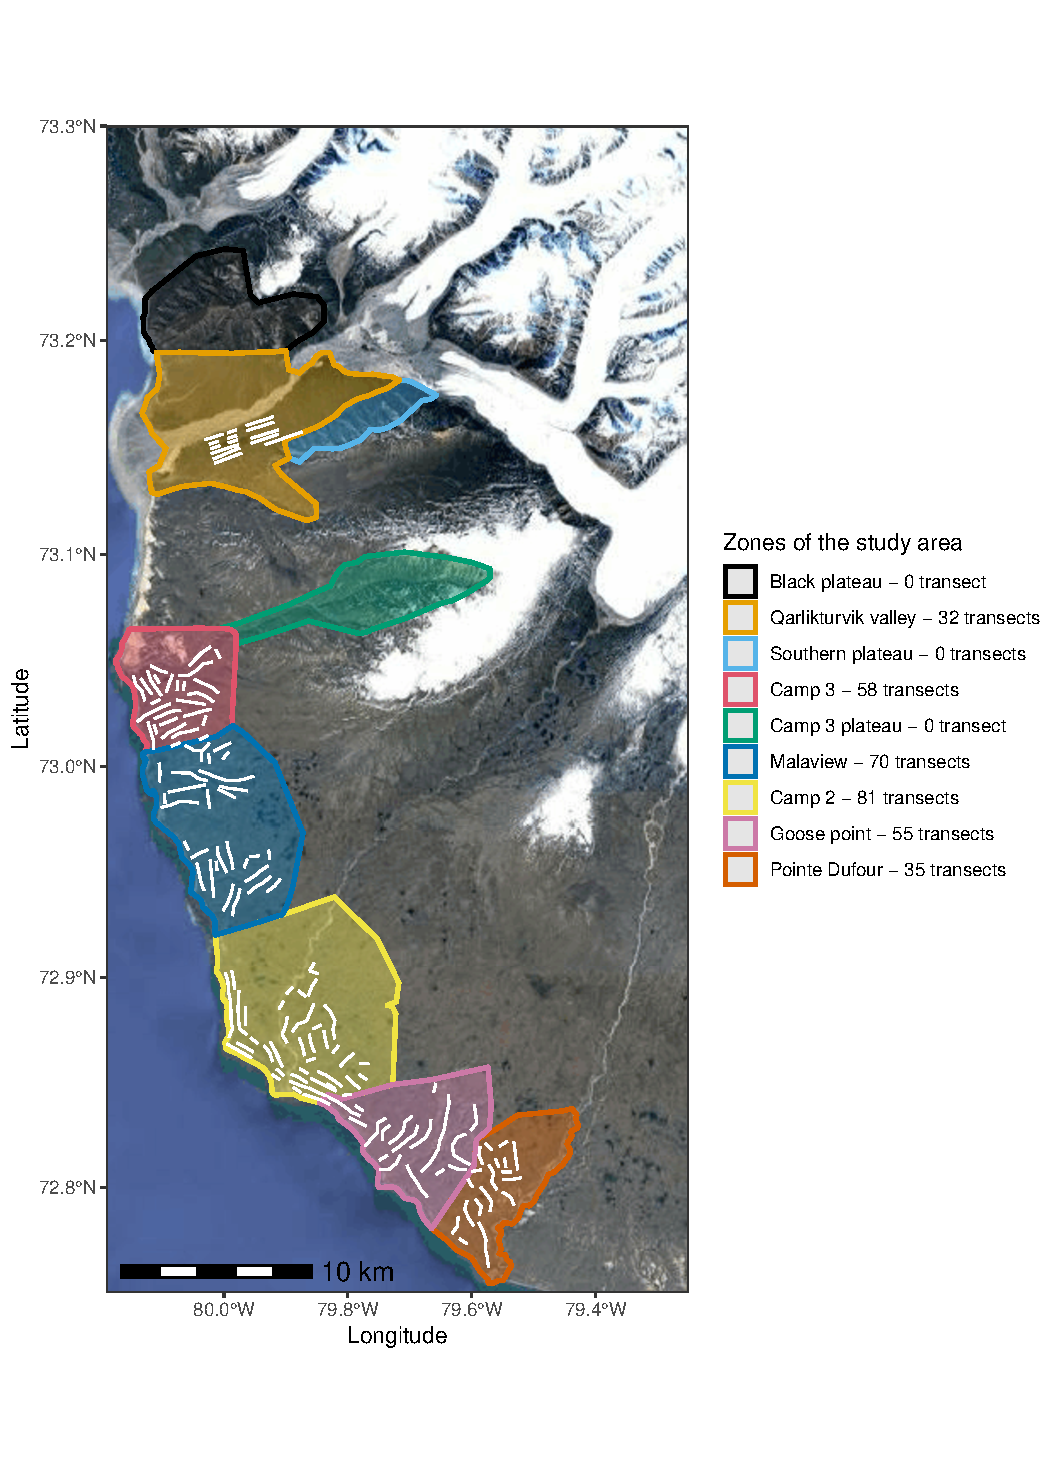
\includegraphics[width=0.7\textwidth, angle=0]{figures/transects.pdf}
  \vspace{-35pt} % Reduce space between figure and caption
  \caption{Spatial distribution of vertebrate count transects (white lines) on the south plain of Bylot Island (146 to 320 transects per year).}
 \label{figure:transects}
\end{figure}
\newpage
\item[] \textit{\textbf{Snow goose point count}}\\
At the start, middle, and end of each vertebrate count transect, a point count with a radius of 125 meters was conducted to determine the number of snow goose breeding pairs. On average, 613 \textpm{142} point counts were sampled each year, covering an area of 30 \textpm{7} km\textsuperscript{2}.
\\
\item[] \textit{\textbf{Incidental observations}}\\
Since 2007, observers have recorded all vertebrate species observed opportunistically during field work and tallied the total number of individuals at the end of each day \citep{gauthier2020daily, gauthier2024a}. The number of hours spent in the field served as a proxy for the sampling effort. We used the number of individuals observed per hour spent in the field calculated by \citet{gauthier2024a} as an index of relative abundance for each species. Moreover, we separated observations made in lowland from those in upland zones to have a relative abundance of each species in each of these two broad categories (\textbf{Table \ref{table:table_species_relative_abundance_upland}}). Given that incidental observations lacked georeferencing, we opted to extract upland observations by focusing on observations made during visits to rough-legged hawk nests, which are mostly located in uplands. \\
% latex table generated in R 4.4.1 by xtable 1.8-4 package
% Fri Nov  8 08:10:06 2024
\begin{table}[ht]
\centering
\caption{Index of relative abundance (i.e., number of individuals observed per hour) derived from incidental daily observations for selected vertebrate species in lowland (i.e., Qarlikturvik valley, Camp 3, Malaview, Camp 2, Goose point and Pointe Dufour) and upland (i.e., Black plateau, Southern plateau and Camp 3 plateau) zones of the Bylot Island study area. The ratio compares relative abundance indexes between these two types of zones, calculated by dividing the upland by the lowland index of relative abundance.} 
\label{table:table_species_relative_abundance_upland}
\begingroup\fontsize{10pt}{10pt}\selectfont
\begin{tabularx}{0.55\textwidth}{lrll}
  \hline
  & \multicolumn{2}{c}{Individuals/hour} \\
 Species & Upland & Lowland & Ratio \\
 \hline
Rock ptarmigan & 0.03 & 0.03 & 1 \\ 
  Sandhill crane & 0.42 & 0.287 & 1.5 \\ 
  American golden-plover & 0.26 & 0.394 & 0.7 \\ 
  Black-bellied plover & 0.02 & 0.032 & 0.6 \\ 
  Ruddy turnstone & 0.01 & 0.007 & 1.3 \\ 
  Red knot & 0.00 & 0.033 & 0 \\ 
  Pectoral sandpiper & 0.02 & 0.034 & 0.6 \\ 
  Baird's sandpiper & 0.31 & 0.32 & 1 \\ 
  White-rumped sandpiper & 0.04 & 0.137 & 0.3 \\ 
  Buff-breasted sandpiper & 0.00 & 0.001 & 0 \\ 
  Red phalarope & 0.01 & 0.038 & 0.2 \\ 
  Horned lark & 0.24 & 0.154 & 1.6 \\ 
  American pipit & 0.34 & 0.024 & 14.2 \\ 
  Lapland longspur & 1.93 & 2.641 & 0.7 \\ 
  Snow bunting & 0.59 & 0.092 & 6.4 \\ 
  Arctic hare & 0.02 & 0.009 & 2 \\ 
   \hline
\end{tabularx}
\endgroup
\end{table}

%label-> table_species_relative_abundance_upland
\newpage
\item[] \textit{\textbf{Testimonials of ermine sightings}}\\
There was no direct estimation of ermine abundance on Bylot Island as they are quite difficult to obtain. The density estimates for ermine were derived from an annual abundance index established by \citet{bolduc2023}, which relied on testimonials provided by observers across the whole study area from 1993 to 2019. The testimonials provided by observers were used to create an abundance index ranging from 0 to 3 \citep{bolduc2023}. In this index, a score of 0 corresponds to the absence of ermine sightings, 1 indicates a single sighting of a lone individual, 2 represents multiple sightings of lone individuals, and 3 signifies at least one sighting of a family group. Scores of individual participants were averaged annually as detailed in \citet{bolduc2023}. 
\end{enumerate}
\subsubsection*{d. Capture of individuals}
\begin{enumerate}[label=\roman*]
\item[] \textit{\textbf{Lemming trapping}}\\
Since 2004, Nearctic brown and collared lemmings were live-trapped 3 times during the summer (mid-June, mid-July, and mid-August) in two 11 ha grids. Each grid is made of 144 traps separated by 30 m according to a cartesian plane, one in mesic habitat and the other in wet habitat, located in the Qarlikturvik valley \citep{fauteux2015, gauthier2020lemmings}. Density of each species was estimated at each occasion using spatially explicit capture-recapture methods (see \citet{fauteux2015} for details). From 1995 to 2016 snap-trapping was performed once a year (mid-July) along 2 groups of transects located in the same habitats than the trapping grids \citep{gruyer2008}. Index of abundance derived from snap-trapping were transformed in density estimates in each habitat for the period 1995-2003 using the equation provided by \citet{fauteux2018} based on the period of overlap between the two sampling methods (2004 to 2016). 
\\
\item[] \textit{\textbf{Arctic fox movement tracking}}\\
In order to assess fox abundance based on the size of their home range, 109 Arctic foxes were fitted with Argos Platform Transmitter Terminals mounted on collars between 2008 and 2016 \citep{lai2015,christin2015, dulude2023}. Foxes were captured between May and August across the study area, within and outside the goose colony \citep{dulude2023}. Sampling of animal locations was set for an interval of 1 or 2 days and only locations between May 1 and October 30 were retained \citep{dulude2023}.
\\
\item[] \textit{\textbf{Parasitic jaeger banding}}\\
In 2009, a significant effort was made to band as many parasitic jaegers as possible within the study area. This effort resulted in the banding of 17 adult individuals (Therrien and Gauthier, unpublished data).
\end{enumerate}
\subsubsection*{e. Species body mass}
All vertebrate individuals captured for marking purposes were systematically weighed: snow goose (G. Gauthier, M.-C. Cadieux and J. Lefebvre, unpublished data), snowy owl \citep{therrien2012, robillard2018}, American-golden plovers \citep{lamarre2021}, common-ringed plovers \citep{leandri2019}, other shorebirds (J. Bêty, unpublished data), glaucous gulls \citep{gauthier2015}, long-tailed jaeger \citep{seyer2019}, parasitic jaegers (J.-F. Therrien and G. Gauthier, unpublished data), Lapland longspurs (J. Bêty and G. Gauthier, unpublished data), lemmings \citep{gauthier2020lemmings}, American ermine (Bilodeau and Bolduc, unpublished data) and Arctic foxes \citep{lai2015}. When not available, we extracted mean body mass from the literature \citep{wilman2014}.
\newpage
                        
    \subsection*{3.  Research methods}
                \subsubsection*{a. Field/laboratory}
We estimated the abundance of breeding individuals for most species, but there were a few exceptions. For common ravens, parasitic jaegers, long-tailed ducks, and king eiders, we suspect the presence of a significant number of non-breeding individuals in the study area. Therefore, the estimates we provided for these species include both breeding and potentially non-breeding individuals. Additionally, we did not distinguish between breeding and non-breeding individuals for mammals such as brown and collared lemmings, Arctic fox, American ermine, and Arctic hare. The methods used for each species are summarized in (\textbf{Table \ref{table:table_summary_methods_and_abundance}}).

        \begin{enumerate}[label=\alph*.]       
     \item[] \textit{\textbf{Pacific loon, red-throated loon, cackling goose, tundra swan and glaucous gull}}   \\
Based on the systematic and intensive search for the glaucous gull, cackling goose, tundra swan, red- throated loon and Pacific loon nests in wetlands, we are confident that we have found nearly all nests across the study area from 2017 to 2019 and in 2022. We observed a relatively strong correlation between the nest density of glaucous gulls in the Qarlikturvik valley and the nest density across the entire study area (R\textsuperscript{2}= 0.84, p = 0.16, n= 4). Consequently, we estimated the density of glaucous gulls at the scale of the study area between 2004 and 2016 based on the nest density in the Qarlikturvik valley ($y = 0.12409x + 0.13774$). However, we did not observe such strong relationships for loons and swans and thus we did not extend the time series. Regarding cackling geese, we observed signs of an exponential increase over time based on the annual number of nests found in various zones of the study area. We thus fitted an exponential model using the number of nests found annually over two distinct periods: in 1996 when the first nest was discovered, and then from 2017 to 2023 when sampling effort was systematic across the whole study area (\textbf{Figure \ref{figure:cackling}}). We used the fitted model to estimate abundance between 1996 and 2016 when monitoring was less systematic, which could potentially underestimate observed abundance as seen on \textbf{Figure \ref{figure:cackling}}. We multiplied nest density by two to obtain the abundance (assuming two individuals per nest). 

\begin{figure}[h]
\centering
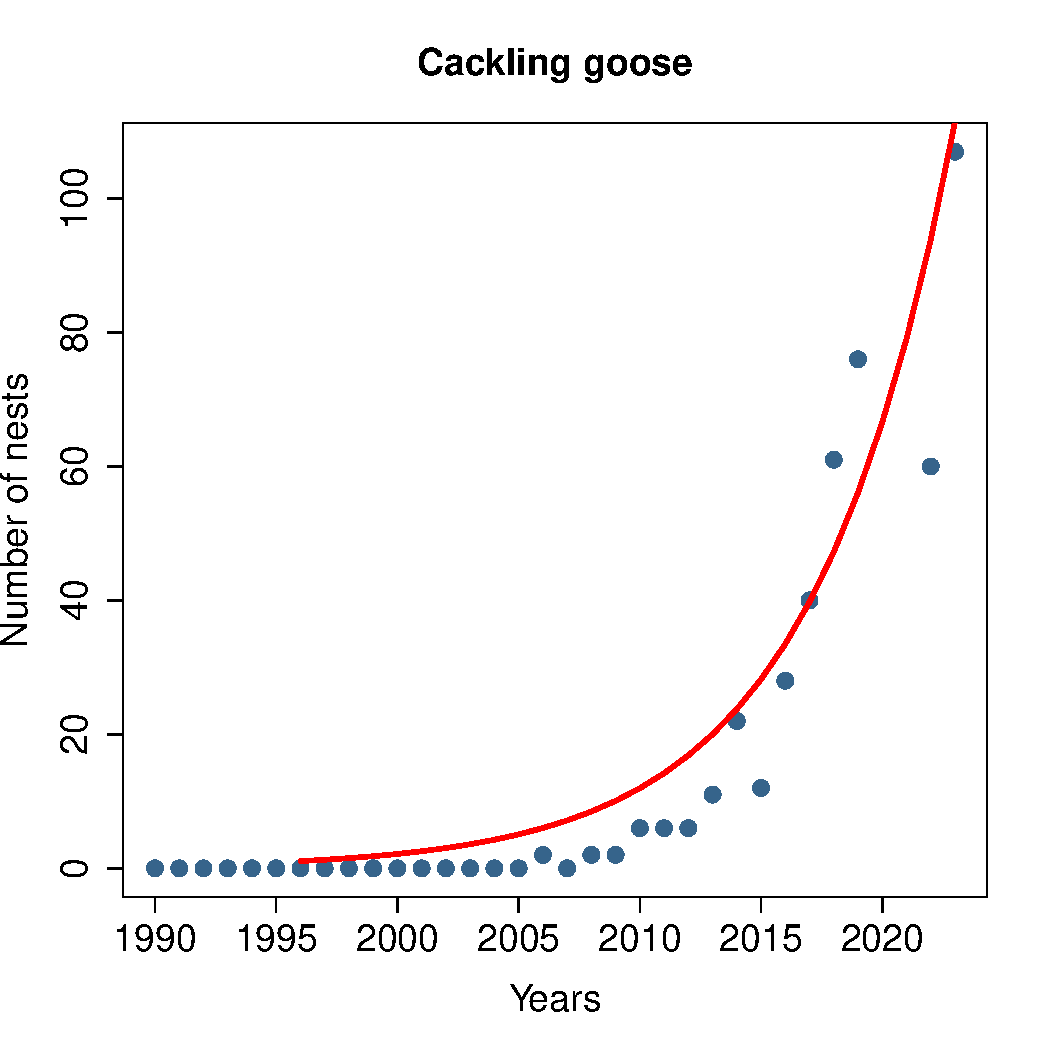
\includegraphics[width=0.6\linewidth]{figures/cackling_goose_nest_exponential.pdf} 
\caption{Number of cackling goose nests found across the study area over time. The red line represents the fitted model over the period 1996-2023 ($y= e^{0.1717x-342.684}$), which was used to estimate the annual abundance of cackling goose between 1996 and 2016. The model presents a strong visual fit with the number of nests found between 2017 and 2023, when nest monitoring was systematic across the study area.}
\label{figure:cackling}
\end{figure}

      \item[] \textit{\textbf{Snow goose}}\\
       Between 1999 and 2023, we assessed the abundance of snow geese in the study area through a multi-step process. We calculated the mean annual density of snow goose nests separately in the mesic and wetland habitats of the area occupied by the goose colony annually. We made slight adjustments to the goose colony perimeter defined from helicopter flights to include all snow goose point counts where at least one breeding pair had been observed (\textbf{Figure \ref{figure:sngo_goose_colony}}). To determine the mean density of nesting geese in wetlands, we divided two times (assuming two individuals per nest) the total number of nests found during systematic nest searches by the total area of wetlands sampled. The density of geese nesting in mesic habitat, a less preferred nesting habitat \citep{lecomte2008}, was averaged from three independent methods: systematic nest searches, vertebrate count transects, and snow goose point counts. Systematic nest searches were highly precise, but covered a relatively small area, whereas transects and snow goose point counts were less precise but covered larger areas. For each method, we calculated the mean density of breeding individuals in mesic habitat by dividing the number of birds (or nests) recorded by the area sampled. Despite methodological differences, the three approaches showed similar inter-annual variations, supporting the use of a mean values to estimate nest density in mesic habitat \textbf{Figure \ref{figure:sngo_interannual_variation}}). Lastly, to transform the densities in total abundance, we determined the annual proportion of wetland and mesic habitats within the goose colony and multiplied the area of each habitat by the density of breeding individuals. For the period 1999 to 2009, we used the average limits of the colony over the period 2010 to 2023 because we did not conduct aerial survey of the colony. Moreover, nest density in the mesic habitat was derived from a single method (\textbf{Figure \ref{figure:sngo_interannual_variation}}). 
                        
        \begin{figure}[ht]
        \centering
        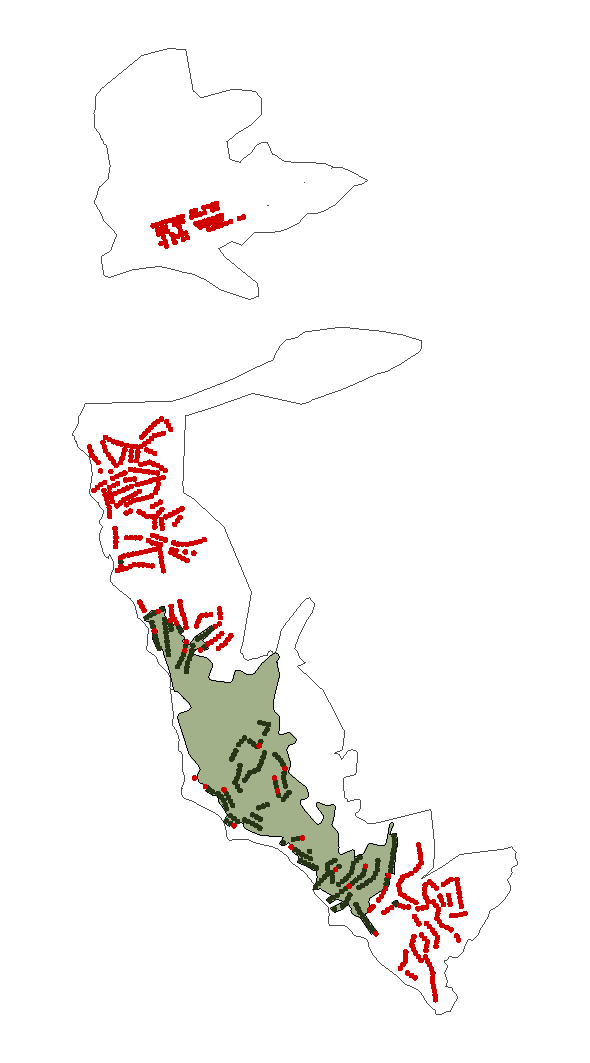
\includegraphics[width=0.5\linewidth]{figures/map_geese_colony_2017.pdf}
        \caption{Map showing the region occupied by the snow goose colony in 2017 (green polygon) as an example. The perimeter was first defined opportunistically using a GPS receiver aboard a helicopter, taking advantage of regular flights across the study area whenever the flight path passed over the colony border. The perimeter was then slightly adjusted to include all snow goose point counts where at least one breeding pair had been observed in that year (green dots). Snow goose point counts where no breeding geese were observed in that year are presented as red dots.}
        \label{figure:sngo_goose_colony}
        \end{figure}
        
        \begin{figure}[ht]
        \centering
        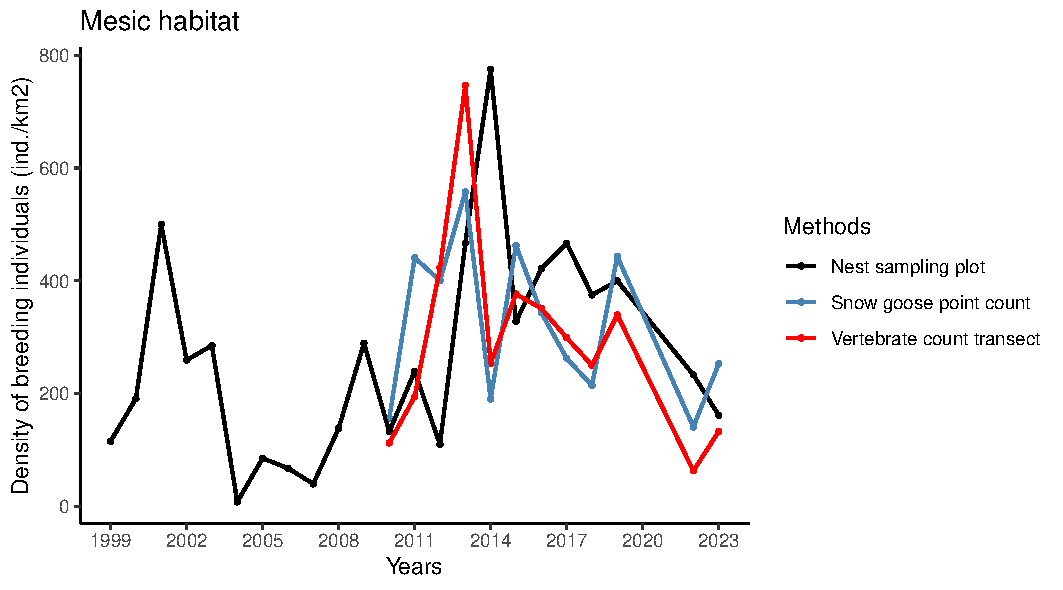
\includegraphics[width=\linewidth]{figures/snow_goose_mesic_density.pdf}
        \caption{Estimates of breeding goose density in mesic habitat within the Bylot Island snow goose colony using three independent methods: Nest sampling plot, Snow goose point count, Vertebrate count transect.}
        \label{figure:sngo_interannual_variation}
        \end{figure}
        \newpage
                                
                \item[] \textit{\textbf{King eider and long-tailed duck}}\\
                We first estimated the abundance of both king eiders and long-tailed ducks based on the annual nest density of each species found in the 8 km\textsuperscript{2} extensive nest search area located in the Qarlikturvik valley. We extrapolated the mean nest density in the wetlands of the Qarlikturvik valley to the wetlands of the study area (38.35 km\textsuperscript{2}). We transformed nest density to abundance of breeding individuals by multiplying it by a factor of two (assuming two individuals per nest). We acknowledge that the opportunistic monitoring of these species likely underestimated their true nest density. However, considering the extensive sampling effort deployed annually within this area, we are confident to obtain a realistic order of magnitude for the number of nests present. Because duck sightings are frequent throughout the breeding period, yet only a few nests are found, we believe there may be a significant portion of non-breeding individuals. Therefore, we employed an additional method to estimate the overall duck populations without differentiating between breeding and non-breeding individuals. 
As an alternative approach, we estimated the abundance of ducks based on the indices of relative abundance (i.e., the number of individuals observed per 100 hours) presented by \citet{gauthier2024a}. We assumed that the ratios between relative and actual abundance are the same (i.e., similar detection probability) in duck and loon species. We therefore derived the absolute abundance of long-tailed ducks and king eiders from their relative abundances using the ratio between relative and absolute abundances of red-throated loons as a reference.
                                
                                
                \item[] \textit{\textbf{Rough-legged hawk, peregrine falcon and snowy owl}} \\
                We estimated the abundance of breeding rough-legged hawks, peregrine falcons and snowy owls based on systematic nest monitoring conducted throughout the study area for these species. To convert the number of nests into breeding abundance, we multiplied it by two (assuming two individuals per nest). For snowy owls, we extended the time series from 1996 to 2011 based on a linear regression between nest density in the Qarlikturvik valley and nearby plateaus (Black and Southern plateaus) and nest density across the entire study area ($y= 0.68867x -0.00173$; R\textsuperscript{2}= 0.99; p < 0.0001, n= 10). We used the same approach for rough-legged hawks ($y=0.49851x$, R\textsuperscript{2}= 0.99, p < 0.0001, n= 8) to extend the time series from 2007 to 2012. We did not extend the time series for peregrine falcons because the correlation is not as strong (R\textsuperscript{2}= 0.44, p= 0.27, n=8).
                
                \item[] \textit{\textbf{Rock ptarmigan}}\\
                We estimated the abundance of rock ptarmigans based on the annual nest density measured in the 8 km\textsuperscript{2} extensive nest search area of the Qarlikturvik valley. While we acknowledge that the opportunistic monitoring of this species likely underestimates nest density, the extensive sampling effort deployed annually within this area gives us confidence in obtaining a realistic number of nests. We then extrapolate the density to the whole study area, without distinction between mesic, wetland and upland habitats (\textbf{Table \ref{table:table_species_relative_abundance_upland}}). Among the 6 nests found in the study area, 4 were located in mesic habitat, while one nest was found in a wetland and another in an upland habitat. To convert the number of nests into breeding abundance, we multiplied it by two (assuming two individuals per nest).
                
                \item[] \textit{\textbf{Sandhill crane}}\\
                We estimated the mean abundance of sandhill cranes in the lowland zones of the study area based on a regression between nest density and the number of individuals observed per transect (\textbf{Figure \ref{figure:sacr}}). In this relationship, nest density and transect observations come from the 8 km\textsuperscript{2} area of the Qarlikturvik valley where extensive nest search is performed. We acknowledge that the opportunistic monitoring of this species likely underestimated the true nest density. However, considering the extensive sampling effort deployed annually within this area, we are confident in obtaining a realistic order of magnitude for the number of nests present. Number of individuals observed along transects in each lowland zone was converted into nest density using the regressions, and then in total number of individuals in each zone by multiplying by the area of the zone and a factor 2. We estimated the density in the upland zones by applying a correction factor to the annual mean density in lowland zones. This correction factor was based on the relative abundance ratio between the upland and lowland zones (\textbf{Table \ref{table:table_species_relative_abundance_upland}}). 
                
\begin{figure}[H]
\centering
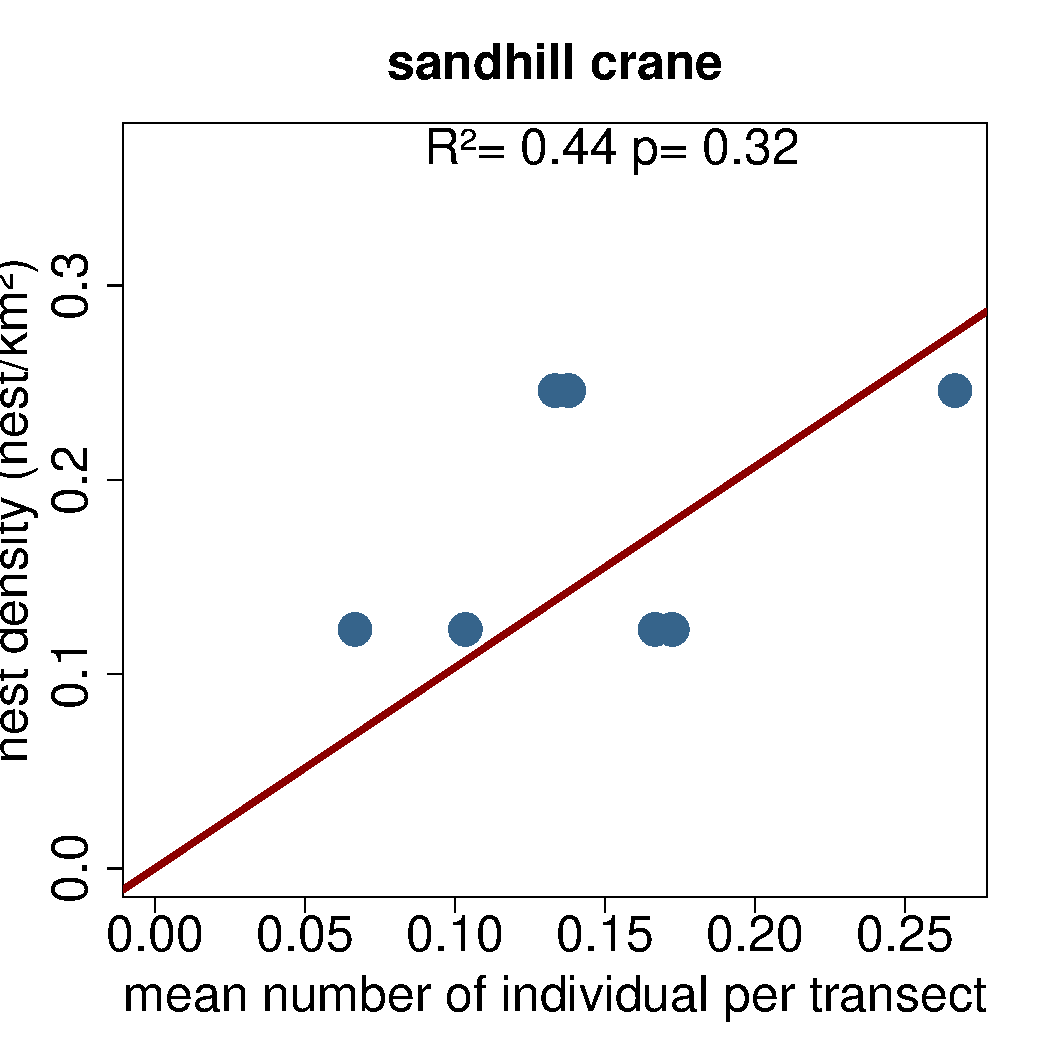
\includegraphics[width=0.5\linewidth]{figures/sandhill_crane_nest_transects.pdf} 
\caption{Linear regression between the nest density of sandhill cranes and the number of individuals observed per transect (nest density = 1.12 x number of individuals per transect; regression was forced to pass through the origin). The fit (R\textsuperscript{2} and p value) of the regression (red line) with the empirical data from the Qarlikturvik valley is presented (blue dots). Data points represent annual values.}
\label{figure:sacr}
\end{figure}
                \item[] \textit{\textbf{American golden-plover and black-bellied plover}}\\
                We used a distance sampling approach to estimate the abundance of American golden-plovers in the lowland zones of the study area between 2014 and 2023. Observations of plovers were made along vertebrate count transects mainly in mesic habitat. Perpendicular distance between detected individuals and the transect path were used (n= 1015) to estimate a detection function with the \textit{ds} function from the \textit{Distance} package \citep{miller2019}. To determine the detection function, we applied a truncation distance of 150 m (i.e., maximum distance on either side of the observer where observations have been considered) and selected the model with the lowest AIC, which included a "hn" key and a single "cos" adjustment term. We excluded observations of groups with more than four individuals, as these likely indicated groups of non-breeders. We did not estimate abundance in wetland habitat because American golden-plovers nest almost exclusively in mesic habitat \citep{parmelee1967}. We estimated the abundance in the upland zones (i.e., plateaus) by applying a correction factor to the abundance in lowland zones. This correction factor was based on the relative abundance ratio between the upland and lowland zones (\textbf{Table \ref{table:table_species_relative_abundance_upland}}).
                
To determine the abundance of black-bellied plovers, we used the mean number of black-bellied plovers and American golden-plovers observed per transect as an index of relative abundance. We assumed that the ratios between relative and actual abundance are the same (i.e., similar detection probability) among those species. This assumption is realistic as those species present similarities in size, color, and reproductive behavior. We therefore derived the absolute abundance of black-bellied plovers from their relative abundance using the ratio between relative and absolute abundances of American golden-plover as a reference. As an alternative approach to determine black-bellied plover abundance, we used the same approach as previously described, but with the indices of relative abundance presented by \citet{gauthier2024a}, which was derived from incidental daily observations.

                \item[] \textit{\textbf{Common-ringed plover}}\\
                To estimate the abundance of common-ringed plovers in the study area, we relied on the total number of nests recorded annually from 2015 to 2017, during which the primary nesting sites underwent intensive sampling. We multiplied the total nest count by two to represent the abundance of breeding individuals (assuming two individuals per nest).
                
                \item[] \textit{\textbf{Lapland longspur and Baird’s sandpiper}}\\
                We estimated the mean abundance of Lapland longspur in the different lowland zones of the study area based on a regression between nest density and the number of individuals observed per transect (\textbf{Figure \ref{figure:lalo_basa}}). For Baird’s sandpiper, we employed a similar approach, but instead of using the mean number of individuals observed per transect, we used the mean proportion of transects where at least one individual was detected. We made this adjustment because this species was less frequently observed. In this relationship, nest density for these two species came from the intensive nest sampling conducted within the core 2 km\textsuperscript{2} area of the Qarlikturvik valley and observations of individuals from transects carried out in the larger 8 km\textsuperscript{2} area in which the core area was located. This approach allowed us to incorporate a larger sample size from the transects while focusing on a measure of nest density determined systematically. Transects observations in lowland were then converted into nest density using the regressions, and then in total number of individuals by multiplying by the area and a factor 2. We estimated the density of both species in the upland zones by applying a correction factor to the annual mean density in lowland zones. This correction factor was based on the relative abundance ratio between the upland and lowland zones (\textbf{Table \ref{table:table_species_relative_abundance_upland}}). We acknowledge that the regression for Baird’s sandpiper is weak; however, it offers some refinement compared to assuming a uniform density throughout the study area. 
                
                \begin{figure}[H]
                \begin{subfigure}{0.5\textwidth}
                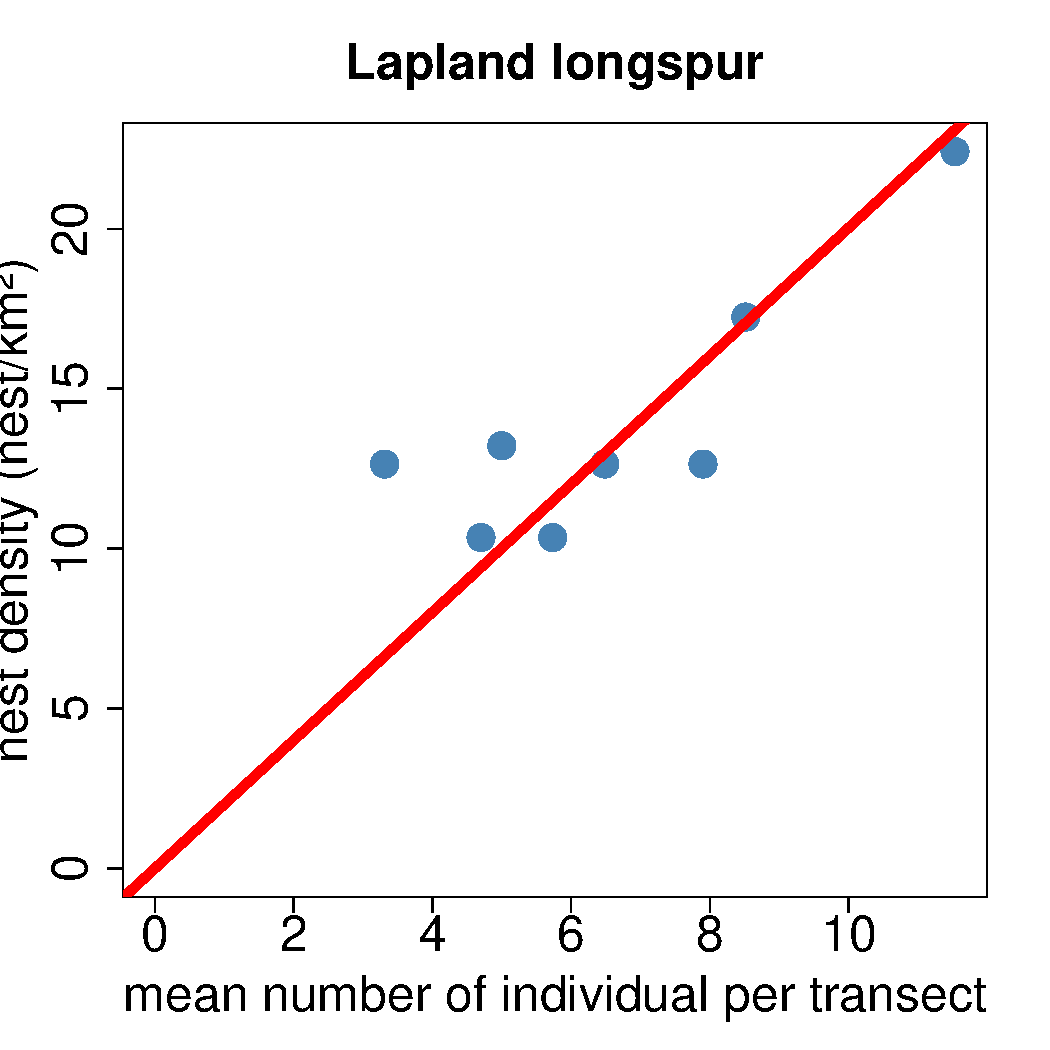
\includegraphics[width=0.95\linewidth]{figures/lapland_longspur_nest_transect.pdf} 
                \caption{}
                \end{subfigure}
                \begin{subfigure}{0.5\textwidth}
                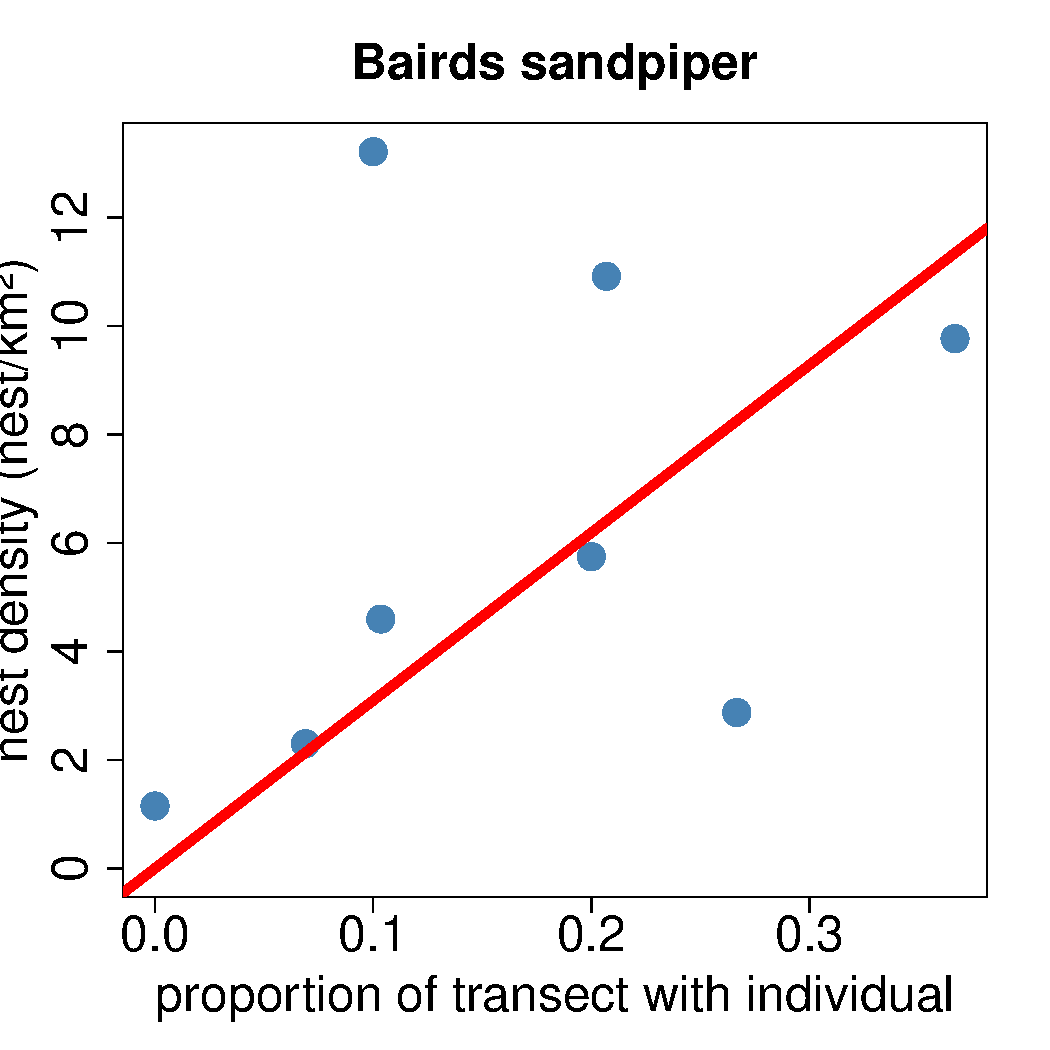
\includegraphics[width=0.95\linewidth]{figures/bairds_sandpiper_nest_transect.pdf}
                \caption{}
                \end{subfigure}
                \caption{a) Linear regression between the nest density of Lapland longspurs and the number of individuals observed per transect (nest density= 2.3422 x number of individuals per transect; regression was forced through the origin). The fit (R\textsuperscript{2} and p value) of the regression (red line) with the empirical data from the Qarlikturvik valley is presented (blue dots). Data points represent annual values. b) Linear regression between the nest density of Baird’s sandpiper and the proportion of transect with at least one individual observed (nest density= 34.9248 x proportion of transects with at least one individual; regression was forced through the origin). The fit (R\textsuperscript{2} and p value) of the regression (red line) with the empirical data from the Qarlikturvik valley is presented (blue dots). Data points represent annual values.}
                \label{figure:lalo_basa}
                \end{figure} 
                
                \item[] \textit{\textbf{Other passerines and sandpipers}}\\
                We estimated the abundance of other passerines (horned lark, American pipit, and snow bunting) in the lowland zones of the study area with the regression equation between number of individuals per transect and nest density of the Lapland longspur (see section \textit{Lapland longspur and Baird’s sandpiper}). We assumed here a similar detection probability for all species. We used the same approach for other sandpiper species (white-rumped sandpiper, pectoral sandpiper, buff-breasted sandpiper, red knot, ruddy turnstone and red phalarope) based on the regression equation for the Baird's sandpiper (see section \textit{Lapland longspur and Baird’s sandpiper}). For all these species, we estimated the density in the upland zones by applying a correction factor to the mean density in lowland zones. This correction factor was based on the relative abundance ratio between the upland and lowland zones (\textbf{Table \ref{table:table_species_relative_abundance_upland}}). Nest density was then converted in number of individuals by multiplying by the area and a factor 2.
As an alternative approach, we estimated the abundance of other passerines and sandpipers based on the indices of relative abundance (i.e., the number of individuals observed per 100 hours) presented by \citet{gauthier2024a}. We assumed that the ratios between relative and actual abundance are the same (i.e., similar detection probability) among both passerine and sandpiper species. We therefore derived the absolute abundance of other passerine and sandpiper species from their relative abundances using respectively, the ratios between relative and absolute abundances of Lapland longspur (passerines) and Baird’s sandpiper (sandpipers) as references.

                \item[] \textit{\textbf{Long-tailed jaeger}}\\
                We determined the annual nest density of long-tailed jaegers from the systematic nest sampling between 2004 and 2023 on the southern side of the glacial river in the Qarlikturvik valley. We determined nest density by dividing the annual number of nests recorded by the area of the surveyed zone (33 km\textsuperscript{2}). As long-tailed jaegers typically nest in mesic habitat \citep{andersson1971}, we multiplied the area occupied by mesic habitat across the study area by the nest density obtained in the surveyed zone and by two to obtain the total abundance of breeding individuals (assuming two individuals per nest).
                
                \item[] \textit{\textbf{Parasitic jaeger}}\\
                Based on the opportunistic nest monitoring of parasitic jaegers across the study area, an average of 4 nests is found annually, a small number considering that parasitic jaegers were frequently observed at the study site \citep{gauthier2024a}. This suggests that there may be non-breeding individuals present at the study site, or alternatively, individuals may regularly travel long distances, potentially from outside the study area, to forage during the breeding season. Due to limited data availability for estimating the abundance of non-breeding parasitic jaegers, we relied on the maximum number of adults banded during a single year (17 individuals in 2009; Therrien, unpublished data) as the minimum abundance on the study area. This corresponds to a density of 0.04 individuals/km\textsuperscript{2}. For comparison, \citet{taylor1974} measured a density of 0.06 individual/km\textsuperscript{2} on Bathurst Island.
                
                \item[] \textit{\textbf{Common raven}}\\
                Despite the intensive nest searches for raptors in upland zones, we never found more than one common raven nest each year, a small number considering the frequent raven observations at the study site \citep{gauthier2024a}. This indicates the potential presence of non-breeding individuals or individuals that breed outside the study area but use it for foraging throughout the breeding period. Therefore, we opted for alternative approaches based on individual counts to estimate the abundance of both breeding and non-breeding ravens. 
As a first approach, we based our estimate of ravens on the number of glaucous gulls observed per transect. We assumed that the ratios between relative and actual abundance are the same (i.e., similar detection probability) among those species. This assumption is reasonable as those species present similarities in size and foraging strategy. We therefore derived the absolute abundance of common ravens from their relative abundance using the ratio between relative and absolute abundances of glaucous gulls as a reference.  
Independently, we estimated the abundance of common ravens with the same approach but using the indices of relative abundance presented by \citet{gauthier2024a}, which was derived from incidental daily observations, rather than observations from the transects.

        \item[] \textit{\textbf{Nearctic brown and collared lemming}}\\
        Between 1995 and 2003, we used the density estimates derived from the snap-trapping indices obtained in late July in each habitat. Between 2004 and 2007, annual abundance of each lemming species was based on the late-July density estimates on trapping grid in wet and mesic habitats. However, starting from 2008, estimates were derived from the mean density recorded in mid-July and mid-August, except for two instances: 2019 and 2021. In 2019, due to an exceptionally early snowmelt and thus an early decline in lemmings during the summer, we only retained value from mid-July. In 2021, we relied solely on data gathered in August because it was the only trapping period carried out that year. To scale the estimated densities from the wet and mesic grids to the entire study area, we used the proportions of mesic habitats (64\%) and wet habitats (10\%) measured within the study area.
        
                \item[] \textit{\textbf{Arctic hare}}\\
                Arctic hares are primarily observed in the upland zones of the study area, where sampling effort is limited. We thus derived abundance of hares from the estimated abundance of Arctic foxes based on indices of relative abundance presented in \citep{gauthier2024a}, which were derived from incidental daily observations. We doubled the density of Arctic hares in the upland zones (i.e., plateaus), as twice as many individuals were observed per hour of fieldwork there compared to lowland zones (\textbf{Table \ref{table:table_species_relative_abundance_upland}}). However, it is worth noting that assuming a similar detection probability between foxes and hares might lead to an overestimation of hare detection probability due to behavioral differences between the species. Therefore, we most likely underestimate the actual abundance of Arctic hares in the study area.
                
                \item[] \textit{\textbf{American ermine}}\\
   				We estimated the annual abundance of ermines by transforming the annual index of relative abundance provided in \citet{bolduc2023} into individual density. Annual values ranged from 0, indicating no ermine sighting, to 2.88, which signifies that nearly all observers observed at least one family group during their field season. We independtly obtained measures of minimum (0.02 ind./km\textsuperscript{2}) and maximum (0.4 ind./km\textsuperscript{2}) ermine density, which were determined from estimates of individual home range obtained from radio-tracking data, observations on Bylot Island, and existing literature \citep{legagneux2012, bilodeau2013}. We associated the minimum and maximum scores of relative abundance with the minimum and maximum density of individuals, respectively. Ultimately, we calculated the ermine density by linearly interpolating between these two density extremes using the annual index of relative abundance.
                
                \item[] \textit{\textbf{Arctic fox}}\\
                We estimated the abundance of Arctic foxes in the study area based on their estimated home range size inside and outside the goose colony. We used the data and methodologies outlined in \citet{dulude2023} to estimate home range size. However, here, we did not account for annual variations in lemming density as presented in \citet{dulude2023} in order to obtain mean fox home range. Given that foxes are territorial and exhibit an average spatial overlap with adjacent territories of 18\% \citep{clermont2021}, we converted home range size into individual density using the following formula: $\text{\textit{density of individuals}}= \frac{2}{0.82\times \text{\textit{home range}}}$. We used two as numerator because we assumed each territory was held by a pair of fox, either breeding or non-breeding fox pair, without accounting for potential nomadic or transient individuals. We used values of 12.26 km\textsuperscript{2} to represent the mean home range of foxes within the goose colony and 20.02 km\textsuperscript{2} for foxes outside the goose colony. We estimated the mean density of foxes in each zone of the study area according to the mean proportion of the zone covered by the goose colony. We derived the mean annual proportion of each zone covered by the goose colony from the colony outline between 2010 and 2023. We estimated a mean density of 0.14 individuals/km\textsuperscript{2} for the study area. Previously, the minimum density of foxes in the study area was estimated to be between 0.03 and 0.13 individuals per km\textsuperscript{2} based on camera traps \citep{royerboutin2015}. 
                \newpage
                        \end{enumerate}
                        
                        \newgeometry{top=0.5cm, bottom=1.5cm, left=0.5cm, right=0.5cm}
\begin{landscape}
% latex table generated in R 4.4.1 by xtable 1.8-4 package
% Fri Oct 25 14:16:25 2024
\begingroup\fontsize{8pt}{10pt}\selectfont
\begin{longtable}{|p{0.10\textwidth}|p{0.27\textwidth}|p{0.06\textwidth}|p{0.23\textwidth}|p{0.09\textwidth}|p{0.09\textwidth}|p{0.085\textwidth}|p{0.04\textwidth}|p{0.10\textwidth}|}
\caption{Summary of the lowest, highest, mean and standard deviation of the estimated abundance of each vertebrate species in the vertebrate community of the southern plain of Bylot Island (389 km2). In some cases, two independent approaches have been used to estimate the abundance of the same species as a proxy for uncertainty. We provide a qualitative measure of the method quality based on data available, method used for extrapolation (if necessary), and in some cases, from the fit of statistical models to estimate density. The star (*) refers to the estimate of breeding individuals only.} \\ 
  \hline
{\textbf{Species}} & {\textbf{Method}} & {\textbf{Method quality}} & {\textbf{Justification}} & {\textbf{Lowest abundance}} & {\textbf{Highest abundance}} & {\textbf{Mean abundance}} & {\textbf{sd}} & {\textbf{n}} \\ 
  \hline
Pacific loon & Intensive study area-wide nest monitoring (389 km2) & high & No extrapolation & 0* & 6* & 4* & 3 & 4 (2017-2019, 2022) \\ 
   \hline
Red-throated loon & Intensive study area-wide nest monitoring (389 km2) & high & No extrapolation & 42* & 76* & 64* & 15 & 4 (2017-2019, 2022) \\ 
   \hline
King eider & Intensive, but opportunistic nest monitoring (8 km2) extrapolated by habitat & very low & Intensive, but opportunistic monitoring at relatively small spatial scale, but does not include potential non-breeding individuals &  &  & 25* &  &  \\ 
   \hline
King eider & Derived from the abundance estimate of red-throated loon using incidental observations & low & Derived from high quality estimate of another species &  &  & 106 &  &  \\ 
   \hline
Long-tailed duck & Intensive, but opportunistic nest monitoring (8 km2) extrapolated by habitat & very low & Intensive, but opportunistic monitoring at relatively small spatial scale, but does not include potential non-breeding individuals &  &  & 20* &  &  \\ 
   \hline
Long-tailed duck & Derived from the abundance estimate of red-throated loon using incidental observations & low & Derived from high quality estimate of another species &  &  & 191 &  &  \\ 
   \hline
Cackling goose & Extrapolation from exponential model of growth (strong visual fit with empirical data) & moderate & Strong correlation with opportunistic nest monitoring & 2* & 158* & 31* & 41 & 23 (1996-2016, 2020-2021) \\ 
   \hline
Cackling goose & Intensive study area-wide nest monitoring (389 km2) & high & No extrapolation & 80* & 214* & 138* & 50 & 5 (2017-2019, 2022-2023) \\ 
   \hline
Snow goose & Nest monitoring plots extrapolated to mean goose colony area & moderate & Relatively small sample size and uncertainty on goose colony area  & 2505* & 35404* & 18129* & 11037 & 11 (1999-2009) \\ 
   \hline
Snow goose & Intensive study area-wide monitoring based on a combination of methods (transects, point counts and nest monitoring plots) and annual colony outline & high & Multiple independent methods and annual colony outline & 7982* & 47859* & 30771* & 11962 & 12 (2010-2019, 2022-2023) \\ 
   \hline
Tundra swan & Intensive study area-wide nest monitoring (389 km2) & high & No extrapolation & 0* & 2* & 1* & 1 & 4 (2017-2019, 2022) \\ 
   \hline
Rough-legged hawk & Extrapolation from intensive nest monitoring (111 km2, R2=0.99, p$<$0.0001, n=8) & high & Strong correlation with study area-wide nest density & 3* & 59* & 22* & 21 & 6 (2007-2012) \\ 
   \hline
Rough-legged hawk & Intensive study area-wide nest monitoring (389 km2) & high & No extrapolation & 0* & 66* & 30* & 29 & 8 (2013-2019, 2022) \\ 
   \hline
Peregrine falcon & Intensive study area-wide nest monitoring (389 km2) & high & No extrapolation & 8* & 12* & 10* & 1 & 8 (2013-2019, 2022) \\ 
   \hline
Snowy owl & Extrapolation from intensive nest monitoring (111 km2, R2=0.99, p$<$0.0001, n=10) & high & Strong correlation with study area-wide nest density &  &  &  &  & NA (1996-2011) \\ 
   \hline
Snowy owl & Intensive study area-wide nest monitoring (389 km2) & high & No extrapolation & 0* & 144* & 17* & 45 & 10 (2012-2019, 2022-2023) \\ 
   \hline
Rock ptarmigan & Intensive, but opportunistic nest monitoring (8 km2) extrapolated to study area & very low & Intensive, but opportunistic monitoring at relatively small spatial scale and prime nesting habitat not well sampled &  &  & 24* &  &  \\ 
   \hline
Sandhill crane & Extrapolation from intensive nest monitoring (8 km2) and transect observations (R2= 0.44 p= 0.32, n=8) & moderate & Uncertain relation with large scale indices &  &  & 34* &  &  \\ 
   \hline
American golden-plover & Distance sampling throughout lowland (313 km2) & high & Large sample size & 397* & 1725* & 1102* & 432 & 8 (2014-2019, 2022-2023) \\ 
   \hline
Black-bellied plover & Derived from the abundance estimate of American golden-plover using transects observations & low & Derived from high quality estimate of another species &  &  & 29* &  &  \\ 
   \hline
Black-bellied plover & Derived from the abundance estimate of American golden-plover using incidental observations & very low & Derived from high quality estimate of another species, but potentially includes transient migratory individuals &  &  & 87* &  &  \\ 
   \hline
Common-ringed plover & Nest monitoring on the main breeding sites & moderate & Intensive monitoring, but not exhaustive to study area & 44* & 62* & 55* & 9 & 3 (2015-2017) \\ 
   \hline
Ruddy turnstone & Derived from the abundance estimate of Bairds sandpiper using transects observations & low & Derived from moderate quality estimate of another species &  &  & 40* &  &  \\ 
   \hline
Ruddy turnstone & Derived from the abundance estimate of Bairds sandpiper using incidental observations & very low & Derived from moderate quality estimate of another species, but potentially includes transient migratory individuals &  &  & 53* &  &  \\ 
   \hline
Red knot & Derived from the abundance estimate of Bairds sandpiper using transects observations & low & Derived from moderate quality estimate of another species &  &  & 66* &  &  \\ 
   \hline
Red knot & Derived from the abundance estimate of Bairds sandpiper using incidental observations & very low & Derived from moderate quality estimate of another species, but potentially includes transient migratory individuals &  &  & 233* &  &  \\ 
   \hline
Pectoral sandpiper & Derived from the abundance estimate of Bairds sandpiper using transects observations & low & Derived from moderate quality estimate of another species &  &  & 80* &  &  \\ 
   \hline
Pectoral sandpiper & Derived from the abundance estimate of Bairds sandpiper using incidental observations & very low & Derived from moderate quality estimate of another species, but potentially includes transient migratory individuals &  &  & 255* &  &  \\ 
   \hline
Baird's sandpiper & Extrapolation from intensive nest monitoring (2 km2) and transects observations (R2=0.38, p=0.35, n=8) & moderate & Uncertain relation with large scale indices &  &  & 2448* &  &  \\ 
   \hline
White-rumped sandpiper & Derived from the abundance estimate of Bairds sandpiper using transects observations & low & Derived from moderate quality estimate of another species &  &  & 991* &  &  \\ 
   \hline
White-rumped sandpiper & Derived from the abundance estimate of Bairds sandpiper using incidental observations & very low & Derived from moderate quality estimate of another species, but potentially includes transient migratory individuals &  &  & 1134* &  &  \\ 
   \hline
Buff-breasted sandpiper & Derived from the abundance estimate of Bairds sandpiper using transects observations & low & Derived from moderate quality estimate of another species &  &  & 6* &  &  \\ 
   \hline
Buff-breasted sandpiper & Derived from the abundance estimate of Bairds sandpiper using incidental observations & very low & Derived from moderate quality estimate of another species, but potentially includes transient migratory individuals &  &  & 8* &  &  \\ 
   \hline
Red phalarope & Derived from the abundance estimate of Bairds sandpiper using transects observations & low & Derived from moderate quality estimate of another species &  &  & 140* &  &  \\ 
   \hline
Red phalarope & Derived from the abundance estimate of Bairds sandpiper using incidental observations & very low & Derived from moderate quality estimate of another species, but potentially includes transient migratory individuals &  &  & 270* &  &  \\ 
   \hline
Glaucous gull & Extrapolation from intensive nest monitoring (111 km2, R2=0.84, p=0.16, n=4) & high & Strong correlation with study area-wide nest density & 59* & 80* & 73* & 6 & 13 (2004-2016) \\ 
   \hline
Glaucous gull & Intensive study area-wide nest monitoring (389 km2) & high & No extrapolation & 60* & 80* & 71* & 9 & 4 (2017-2019, 2022) \\ 
   \hline
Long-tailed jaeger & Intensive nest monitoring (33 km2) extrapolated by habitat & high & Relatively large spatial coverage of sampling & 0* & 900* & 272* & 285 & 17 (2004-2019, 2022) \\ 
   \hline
Parasitic jaeger & Maximum number of individuals banded in a year & low & Based on a single year and potentially not all individuals were captured &  &  & 17 &  &  \\ 
   \hline
Parasitic jaeger & Maximum number of nest found annually during study area-wide opportunistic nest monitoring & very low & Monitoring does not include potential non-breeding individuals &  &  & 8* &  &  \\ 
   \hline
Common raven & Derived from the abundance estimate of glaucous gull using transects observations & very low & Derived from moderate quality estimate of another species, but potential difference in detectability between species &  &  & 14 &  &  \\ 
   \hline
Common raven & Derived from the abundance estimate of glaucous gull using incidental observations & very low & Derived from moderate quality estimate of another species, but potential difference in detectability between species &  &  & 18 &  &  \\ 
   \hline
Horned lark & Derived from the abundance estimate of Lapland longspur using transects observations & low & Derived from moderate quality estimate of another species &  &  & 362* &  &  \\ 
   \hline
Horned lark & Derived from the abundance estimate of Lapland longspur using incidental observations & low & Derived from moderate quality estimate of another species &  &  & 411* &  &  \\ 
   \hline
American pipit & Derived from the abundance estimate of Lapland longspur using transects observations & very low & Derived from moderate quality estimate of another species and prime nesting habitat not sampled &  &  & 53* &  &  \\ 
   \hline
American pipit & Derived from the abundance estimate of Lapland longspur using incidental observations & low & Derived from moderate quality estimate of another species and prime nesting habitat not well sampled &  &  & 87* &  &  \\ 
   \hline
Lapland longspur & Extrapolation from intensive nest monitoring (2 km2) and transects observations (R2=0.62, p=0.1, n=8) & moderate & Uncertain relation with large scale indices &  &  & 7110* &  &  \\ 
   \hline
Snow bunting & Derived from the abundance estimate of Lapland longspur using transects observations & very low & Derived from moderate quality estimate of another species and prime nesting habitat not sampled &  &  & 18* &  &  \\ 
   \hline
Snow bunting & Derived from the abundance estimate of Lapland longspur using incidental observations & low & Derived from moderate quality estimate of another species and prime nesting habitat not well sampled &  &  & 276* &  &  \\ 
   \hline
Nearctic brown lemming & Rigorous density estimates at small spatial scale (0.22 km2) extrapolated by habitat & moderate & Intensive sampling, but small spatial coverage and extrapolation by habitat & 0 & 447630 & 54043 & 93530 & 27 (1995-2019, 2021-2022) \\ 
   \hline
Nearctic collared lemming & Rigorous density estimates at small spatial scale (0.22 km2) extrapolated by habitat & moderate & Intensive sampling, but small spatial coverage and extrapolation by habitat & 0 & 39302 & 8128 & 10334 & 27 (1995-2019, 2021-2022) \\ 
   \hline
Arctic hare & Derived from the abundance estimate of Arctic fox using incidental observations & very low & Derived from moderate quality estimate of another species, prime nesting habitat not well sampled and difference in detectability between species &  &  & 6 &  &  \\ 
   \hline
American ermine & Indices of relative abundance derived from testimonials converted to abundance using home range size & moderate & Indirect indices and uncertainty on ermine home range size estimates & 8 & 156 & 40 & 37 & 27 (1993-2019) \\ 
   \hline
Arctic fox & Derived from extensive fox home range size studies (n=109) & moderate & Indirect indices, but large sample size &  &  & 53 &  &  \\ 
   \hline
\hline
\label{table:table_summary_methods_and_abundance}
\end{longtable}
\endgroup

%label-> table:table_summary_methods_and_abundance
\end{landscape}
\restoregeometry
\newpage
\begin{figure}[h]
\caption{Time series of the estimated annual abundance of vertebrate species on the southern plain of Bylot Island (389 km\textsuperscript{2}). Estimated abundance represents adult individuals, with the exception of lemmings, for which juveniles were also included in the estimate. Time series shorter than 5 years are not presented.}
  \centering
  \begin{subfigure}{0.45\textwidth}
    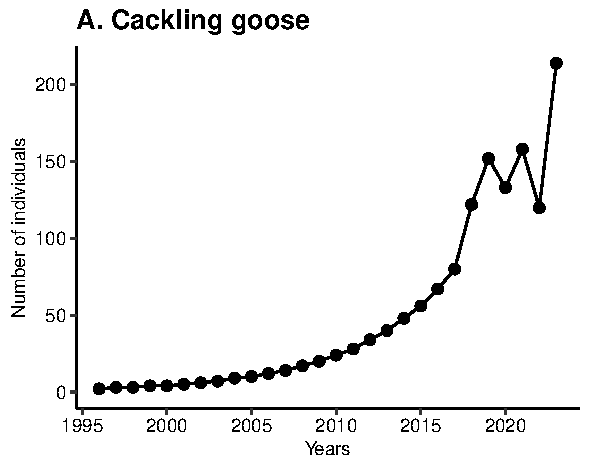
\includegraphics[width=\linewidth]{figures/species_temporal_series/Cackling_goose.pdf}
  \end{subfigure}
  \begin{subfigure}{0.45\textwidth}
    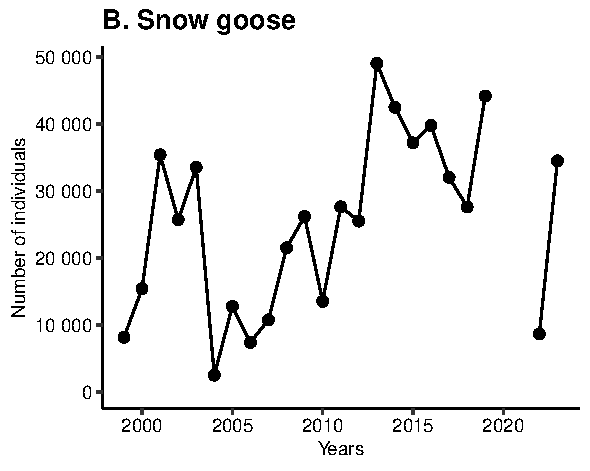
\includegraphics[width=\linewidth]{figures/species_temporal_series/Snow_goose.pdf}
  \end{subfigure} 
    \hfill
    \hfill
  \begin{subfigure}{0.45\textwidth}
    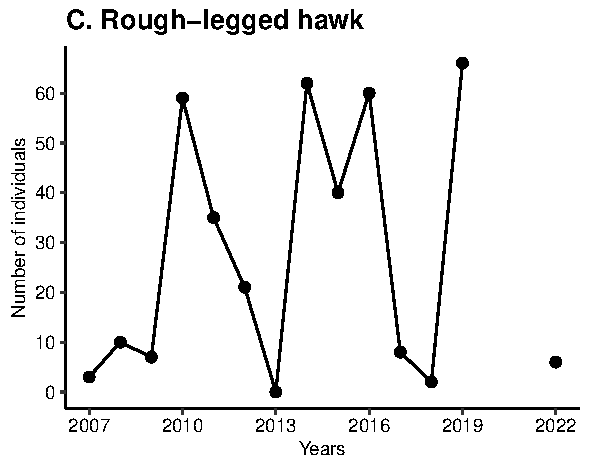
\includegraphics[width=\linewidth]{figures/species_temporal_series/Rough-legged_hawk.pdf}
  \end{subfigure}
  \begin{subfigure}{0.45\textwidth}
    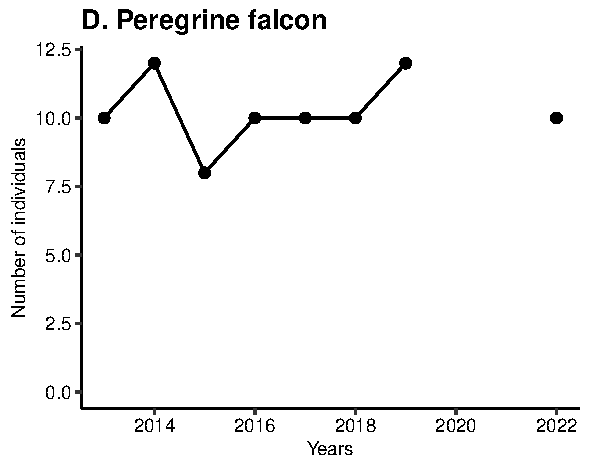
\includegraphics[width=\linewidth]{figures/species_temporal_series/Peregrine_falcon.pdf}
  \end{subfigure}
\end{figure}
\newpage
\begin{figure}[h]
  \centering
  \begin{subfigure}{0.45\textwidth}
    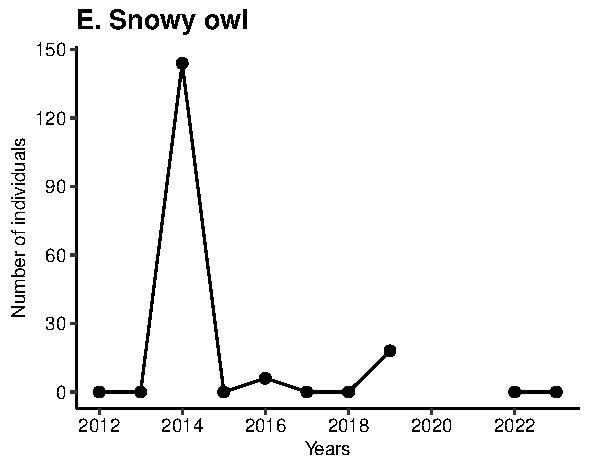
\includegraphics[width=\linewidth]{figures/species_temporal_series/Snowy_owl.pdf}
  \end{subfigure}
  \begin{subfigure}{0.45\textwidth}
    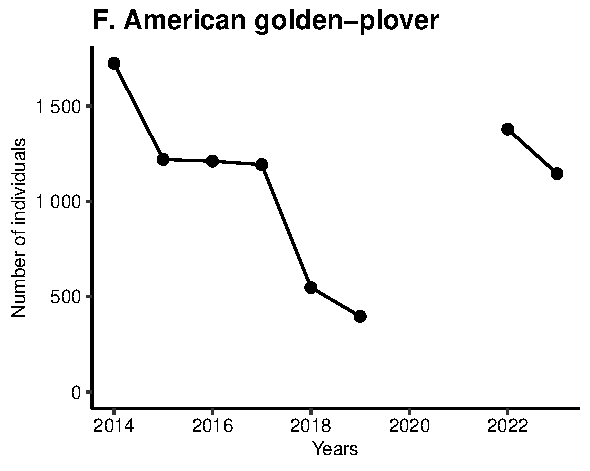
\includegraphics[width=\linewidth]{figures/species_temporal_series/American_golden-plover.pdf}
  \end{subfigure} 
    \hfill
    \hfill
  \begin{subfigure}{0.45\textwidth}
    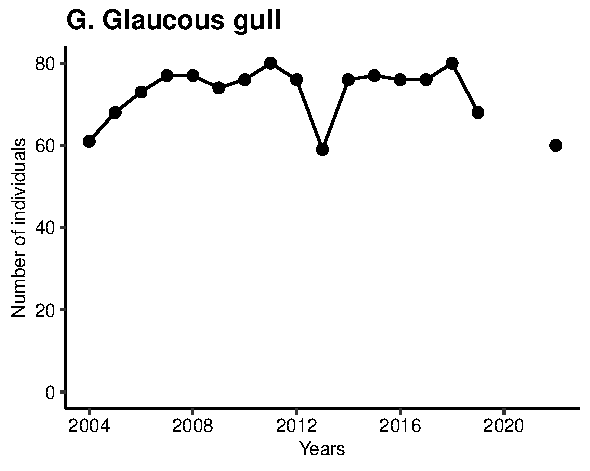
\includegraphics[width=\linewidth]{figures/species_temporal_series/Glaucous_gull.pdf}
  \end{subfigure}
  \begin{subfigure}{0.45\textwidth}
    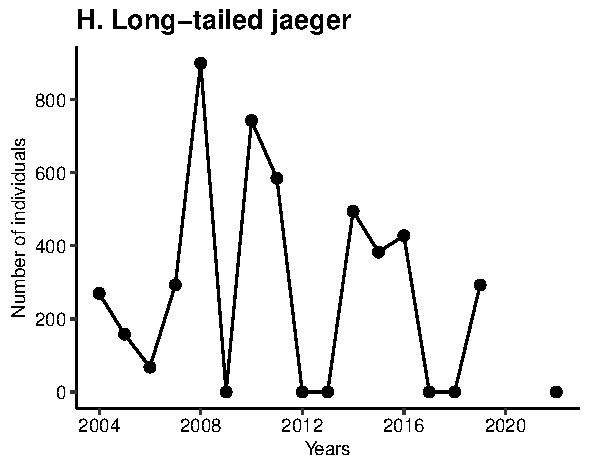
\includegraphics[width=\linewidth]{figures/species_temporal_series/Long-tailed_jaeger.pdf}
  \end{subfigure}
\end{figure}
\newpage
\begin{figure}[h]
  \centering
  \begin{subfigure}{0.45\textwidth}
    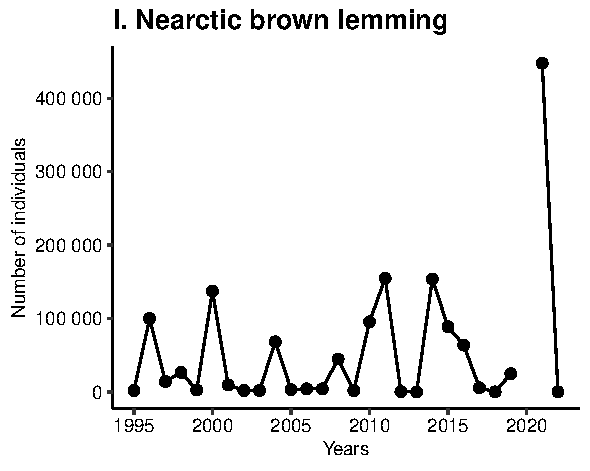
\includegraphics[width=\linewidth]{figures/species_temporal_series/Nearctic_brown_lemming.pdf}
  \end{subfigure}
  \begin{subfigure}{0.45\textwidth}
    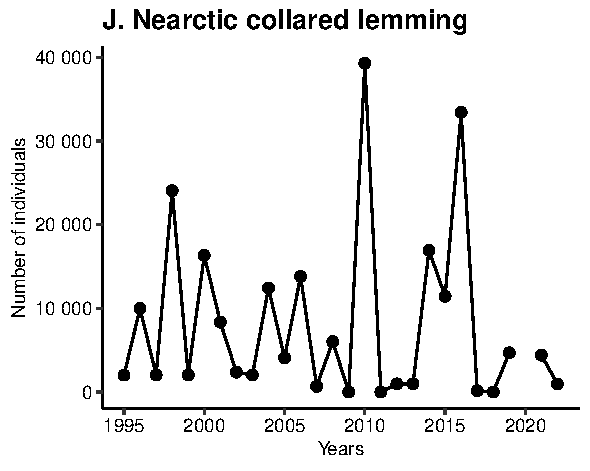
\includegraphics[width=\linewidth]{figures/species_temporal_series/Nearctic_collared_lemming.pdf}
  \end{subfigure} 
    \hfill
    \hfill
  \begin{subfigure}{0.45\textwidth}
    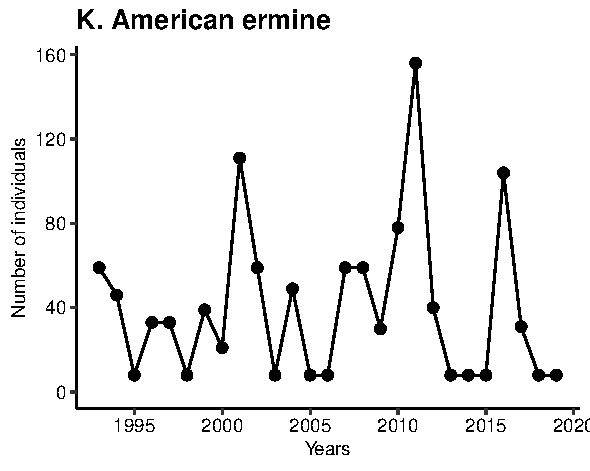
\includegraphics[width=\linewidth]{figures/species_temporal_series/American_ermine.pdf}
  \end{subfigure}
\end{figure}
\newpage
% latex table generated in R 4.4.1 by xtable 1.8-4 package
% Mon Oct  7 11:13:19 2024
\begin{table}[ht]
\centering
\caption{Due to the absence of confidence intervals in our abundance estimates, we present uncertainty intervals based on field expert impressions. These intervals reflect the interval within which experts believe the actual abundance lies. Experts derived these intervals by considering the given abundance estimate, estimates for other species for comparaison, and their field expertise. For species with time series data (several years of estimates), the intervals are presented for the lowest and highest abundance reached within the given time series. For species without time series, the intervals are based on the mean abundance.} 
\begingroup\fontsize{10pt}{8pt}\selectfont
\begin{tabularx}{\textwidth}{lllll}
  \hline
  & &\multicolumn{3}{c}{Annual abundance (individuals)} \\
 Species & Period & Lowest & Highest & Mean \\
 \hline
Snow goose & 1999-2009 & [2500-10000] & [35000-60000] &  \\ 
  Snow goose & 2010-2019, 2022-2023 & [6000-10000] & [45000-60000] &  \\ 
  Snowy owl & 1996-2011 & 0 & [50-100] &  \\ 
  Snowy owl & 2012-2019, 2022-2023 & 0 & [144-170] &  \\ 
  Glaucous gull & 2004-2016 & [50-80] & [70-100] &  \\ 
  Glaucous gull & 2017-2019, 2022 & [60-80] & [80-100] &  \\ 
  Peregrine falcon & 2013-2019, 2022 & [8-12] & [12-20] &  \\ 
  Rough-legged hawk & 2007-2012 & [0-8] & [50-90] &  \\ 
  Rough-legged hawk & 2013-2019, 2022 & [0-4] & [66-86] &  \\ 
  American golden-plover & 2014-2019, 2022-2023 & [100-500] & [1000-2500] &  \\ 
  Cackling goose & 1996-2016, 2020-2021 & [2-10] & [58-220] &  \\ 
  Cackling goose & 2017-2019, 2022-2023 & [80-110] & [214-244] &  \\ 
  Arctic fox & Mean abundance &  &  & [30-60] \\ 
  Nearctic collared lemming & 1995-2019, 2021-2022 & [100-2000] & [20000-50000] &  \\ 
  Nearctic brown lemming & 1995-2019, 2021-2022 & [100-2000] & [200000-450000] &  \\ 
  American ermine & 1993-2019 & [0-10] & [50-156] &  \\ 
  Long-tailed jaeger & 2004-2019, 2022 & [0-10] & [300-900] &  \\ 
  Red-throated loon & 2017-2019, 2022 & [42-62] & [76-96] &  \\ 
  Pacific loon & 2017-2019, 2022 & [0-6] & [6-10] &  \\ 
  Tundra swan & 2017-2019, 2022 & [0-4] & [2-6] &  \\ 
  Common-ringed plover & 2015-2017 & [44-60] & [60-85] &  \\ 
  Black-bellied plover & Mean abundance &  &  & [6-30] \\ 
  Lapland longspur & Mean abundance &  &  & [7000-10000] \\ 
  Baird's sandpiper & Mean abundance &  &  & [1500-3500] \\ 
  Sandhill crane & Mean abundance &  &  & [15-45] \\ 
  King eider & Mean abundance &  &  & [60-250] \\ 
  Long-tailed duck & Mean abundance &  &  & [80-300] \\ 
  Rock ptarmigan & Mean abundance &  &  & [10-60] \\ 
  Horned lark & Mean abundance &  &  & [200-600] \\ 
  Ruddy turnstone & Mean abundance &  &  & [10-30] \\ 
  Red phalarope & Mean abundance &  &  & [20-80] \\ 
  Red knot & Mean abundance &  &  & [10-30] \\ 
  White-rumped sandpiper & Mean abundance &  &  & [1000-2000] \\ 
  Buff-breasted sandpiper & Mean abundance &  &  & [2-10] \\ 
  Pectoral sandpiper & Mean abundance &  &  & [20-100] \\ 
  Parasitic jaeger & Mean abundance &  &  & [15-50] \\ 
  Common raven & Mean abundance &  &  & [30-75] \\ 
  American pipit & Mean abundance &  &  & [50-300] \\ 
  Snow bunting & Mean abundance &  &  & [100-500] \\ 
  Arctic hare & Mean abundance &  &  & [15-50] \\ 
   \hline
\end{tabularx}
\endgroup
\end{table}

%label-> table:table_expert_based_uncertainty
\newpage
                        
                        \subsubsection*{b. Taxonomy and systematics}
Birds taxonomy was obtained from the IOC World Bird List 14.2 \citep{gill2024} and mammals taxonomy from the Mammal species of the world: a taxonomic and geographic reference \citep{MammalDiversityDatabase}.
                        
                        \subsubsection*{c. Permit history}
All research involving animals on Bylot Island has been approved by an institutional Animal Care Committee. In 1999, the study area became part of Sirmiliik National Park, managed by Parks Canada. Since then, all research activities in the park have been approved by a Joint Park Management Committee.
      
                \subsubsection*{d. Project personnel}
                \begin{enumerate}[label=\alph*.]
                        \item[] \textit{\textbf{Principal and associated investigators}}\\
                        Gilles Gauthier, Eric Reed, Jean-François Giroux, Dominique Berteaux, Joël Bêty, Josée Lefebvre, Dominique Gravel, Jean-François Therrien, Nicolas Lecomte, Dominique Fauteux, Pierre Legagneux (see \citet{gauthier2024b})
                        \item[] \textit{\textbf{Students}}\\
                        By combining animal and plant ecology, 24 doctoral theses and 56 master theses have been completed in relation to the study area located on the south plain of Bylot Island (see \citet{gauthier2024b}).
                \end{enumerate}
\newpage 
 \section*{\textcolor{Blue}{Class III. Data set status and accessibility}}
    \section*{A. Status}
                \subsection*{1. Latest update} 30th September 2024
        \subsection*{2. Latest archive date} XXXXXX October 2024
        \subsection*{3. Metadata status} XXXXXX October 2024
        \subsection*{4. Data verification} The methods employed to estimate species abundance were subject to several rounds of revision by the authors.
   \section*{B. Accessibility}
                \subsection*{1. Storage location and medium}
The data set is publicly available at \url{https://datadryad.org/XXXXXXXXXXX}.\\[1.5em]
Raw data and codes used to extract the presented data set are publicly available at \url{https://zenodo.org/XXXXXXXX}.
                 
        \subsection*{2. Contact persons}
        \begin{enumerate}[label=\alph*.]
                        \item[] \textit{\textbf{Overall project}}\\
                        Joël Bêty; \textit{\href{mailto:joel_bety@uqar.ca}{joel{\textunderscore}bety@uqar.ca}}; 418 723-1986 \#1701; 300 allée des Ursulines, Rimouski, Québec, Canada, G5L 3A1, Office B-002
                        \item[] \textit{\textbf{Data and codes}}\\
                         Louis Moisan, \textit{\href{mailto:louis.moisan.bio@gmail.com}{louis.moisan.bio@gmail.com}}
                \end{enumerate}
                \subsection*{3. Copyright restrictions}
                None
                 
                \subsection*{4. Proprietary restrictions}
                        \subsubsection*{a. Release date} None
                        \subsubsection*{b. Citation}
                         Please cite this document when using the data.
                        \subsubsection*{c. Disclaimer} None
                        
                \subsection*{5. Costs}
                None, the data can be used free of charge.          
\newpage
    
 \section*{\textcolor{Blue}{Class IV. Data structural descriptors}}
    \section*{A. Data set file}
                        \subsection*{1. Identity} 
                        a. \texttt{BYLOT-species\_taxonomy.csv}\\
                b. \texttt{BYLOT-species\_abundance.csv}\\
                c. \texttt{BYLOT-species\_body\_mass.csv}\\
                        d. \texttt{BYLOT-interannual\_variation\_nest\_density.csv}\\ 
                        
                        \subsection*{2. Size} 
                        a. 35 records, not including header row (4.3 kB)\\
                        b. 271 records, not including header row  (33.0 kB)\\
                        c. 53 records, not including header row  (3.7 kB)\\
                        d. 18 records, not including header row  (961 B)
                        
                        \subsection*{3. Format and storage mode} All files are in a comma-separated value format (.csv). 
      
                        \subsection*{4. Header information} 
                                \subsubsection*{a. \texttt{BYLOT-species\_taxonomy.csv}}
                                \texttt{class}; \texttt{order}; \texttt{family}; \texttt{genus}; \texttt{species\_scientific}; \texttt{species\_en}; \texttt{species\_fr}; \texttt{species\_code}; \texttt{functional\_group}; \texttt{migratory\_status}
                                
                                \subsubsection*{b. \texttt{BYLOT-species\_abundance.csv}}
                                \texttt{species\_en}; \texttt{year}; \texttt{breeding\_status}; \texttt{abundance}; \texttt{method\_description}; \texttt{method\_quality}
                                
                                \subsubsection*{c. \texttt{BYLOT-species\_body\_mass.csv}}
                                \texttt{species\_en}; \texttt{site};\texttt{mean\_body\_mass\_g}; \texttt{sample\_size}; \texttt{reference}
                                
                                \subsubsection*{d. \texttt{BYLOT-interannual\_variation\_nest\_density.csv}}
                                \texttt{species\_en}; \texttt{zone}; \texttt{mean\_nest\_density\_km2}; \texttt{sd\_nest\_density\_km2}; \texttt{number\_years}
                        
                        \subsection*{5. Alphanumeric attributes} Mixed
                        
                        \subsection*{6. Special characters/fields} Unavailable values are indicated by NA.
                        
                        \subsection*{7. Authentication procedures}
                        Sums of the numeric columns: \\
                        b. \texttt{BYLOT-species\_abundance.csv}: abundance= 2293389\\
                        c. \texttt{BYLOT-species\_body\_mass.csv}: body\_mass\_g= 49617; sample\_size= 13902\\
                        d. \texttt{BYLOT-interannual\_variation\_nest\_density.csv}: mean\_nest\_density\_km2= 19.991; sd\_nest\_density\_km2= 10.539; sample\_size\_nest\_density\_km2= 185
                        
    \section*{B. Variable information}
                \subsection*{1. Variable identity} See Table \ref{table:table_variables_definition}
        \subsection*{2. Variable definition} See Table \ref{table:table_variables_definition}
        \subsection*{3. Units of measurement} See Table \ref{table:table_variables_definition}
        \newpage
        
        % latex table generated in R 4.4.1 by xtable 1.8-4 package
% Thu Oct 10 16:08:07 2024
\begingroup\fontsize{8pt}{10pt}\selectfont
\begin{longtable}{|p{0.08\textwidth}|p{0.21\textwidth}|p{0.50\textwidth}|p{0.08\textwidth}|}
\caption{Summary of variable definition and unit of measurement.} \\ 
  \hline
{\textbf{Data file}} & {\textbf{Variable identity}} & {\textbf{Variable definition}} & {\textbf{Units}} \\ 
  \hline
a. & class & Taxonomic class  for birds (Gill et al., 2024) and mammals species (Upham et al., 2024). & NA \\ 
   \hline
a. & order & Taxonomic order  for birds (Gill et al., 2024) and mammals species (Upham et al., 2024). & NA \\ 
   \hline
a. & family & Taxonomic family  for birds (Gill et al., 2024) and mammals species (Upham et al., 2024). & NA \\ 
   \hline
a. & genus & Taxonomic genus  for birds (Gill et al., 2024) and mammals species (Upham et al., 2024). & NA \\ 
   \hline
a. & species\_scientific & Taxonomic species  for birds (Gill et al., 2024) and mammals species (Upham et al., 2024). & NA \\ 
   \hline
a. & species\_en & Common names of species in English. & NA \\ 
   \hline
a. & species\_fr & Common names of species in French. & NA \\ 
   \hline
a. & functional\_group & Functional group for each species. The classification of species into functional groups is based on Moisan et al. (2023). & NA \\ 
   \hline
a. & migratory\_status & Migratory status of each species. The classification of species migratory status is based on Gauthier et al., (2011)  and Moisan et al. (2023). & NA \\ 
   \hline
b. & species\_en & Common names of species in English. & NA \\ 
   \hline
b. & year & Year corresponding to the estimate of annual abundance. If abundance has not been calculated for a given series of years, but rather as a general average, then NA has been assigned. & years \\ 
   \hline
b. & breeding\_status & Reproductive status of the individuals. & NA \\ 
   \hline
b. & abundance & Estimate of the annual number of individuals found within the 389 km2 study area located on the southern part of Bylot Island during the breeding season (May to August). This includes both breeding and non-breeding individuals that stay in the study area for a significant period of time, and excludes non-breeding individuals that stop for only a few days during their migration. The estimates only consider adults, with the exception of lemmings, for which no distinction has been made between juveniles and adults. & individuals \\ 
   \hline
b. & method\_description & Brief overview of the method used to estimate the species abundance. & NA \\ 
   \hline
b. & method\_quality &  Qualitative measure of the method quality based on data available, method used for extrapolation (if necessary),
and in some cases, from the fit of statistical models to estimate density. & NA \\ 
   \hline
c. & species\_en & Common names of species in English. & NA \\ 
   \hline
c. & site & Site where individual body mass measurements were taken. & NA \\ 
   \hline
c. & mean\_body\_mass\_g & Mean individual body mass. & grams \\ 
   \hline
c. & sample\_size & Number of individuals measured. & individuals \\ 
   \hline
c. & reference & Reference from which estimate of mean body mass were derived. & NA \\ 
   \hline
d. & species\_en & Common names of species in English. & NA \\ 
   \hline
d. & zone & Sampled zone of the study area (see figure 2 and 3). & NA \\ 
   \hline
d. & mean\_nest\_density\_km2 & Estimate of the mean annual nest density measured within the corresponding zone
of the study area. & nests per square kilometer \\ 
   \hline
d. & sd\_nest\_density\_km2 & Standard deviation of the annual nest density measured within the corresponding
zone of the study area. & nests per square kilometer \\ 
   \hline
d. & number\_years & Number of years consider in the calculation of the nest density. & years \\ 
   \hline
\hline
\label{table:table_variables_definition}
\end{longtable}
\endgroup

       \newpage
        
        \subsection*{4. Data type}
                    \subsubsection*{a. Storage type} See Table \ref{table:table_variables_format}
                    \subsubsection*{b. List and definition of variable codes} See Table \ref{table:table_variables_format}
                    \subsubsection*{c. Range for numeric values} See Table \ref{table:table_variables_format}
                    \subsubsection*{d. Missing value codes} Unavailable values are indicated by NA.
                    \subsubsection*{e. Number of digits} See Table \ref{table:table_variables_format}
            \newpage
            
           % latex table generated in R 4.4.1 by xtable 1.8-4 package
% Fri Oct 25 14:20:19 2024
\begingroup\fontsize{8pt}{10pt}\selectfont
\begin{longtable}{|p{0.04\textwidth}|p{0.21\textwidth}|p{0.07\textwidth}|p{0.40\textwidth}|p{0.05\textwidth}|p{0.07\textwidth}|}
\caption{Summary of variable storage type, code definition, range and number of digit.} \\ 
  \hline
{\textbf{Data file}} & {\textbf{Variable identity}} & {\textbf{Storage type}} & {\textbf{Definition variable codes}} & {\textbf{Range}} & {\textbf{Number digits}} \\ 
  \hline
a. & class & string & NA & NA & NA \\ 
   \hline
a. & order & string & NA & NA & NA \\ 
   \hline
a. & family & string & NA & NA & NA \\ 
   \hline
a. & genus & string & NA & NA & NA \\ 
   \hline
a. & species\_scientific & string & NA & NA & NA \\ 
   \hline
a. & species\_en & string & NA & NA & NA \\ 
   \hline
a. & species\_fr & string & NA & NA & NA \\ 
   \hline
a. & functional\_group & string & NA & NA & NA \\ 
   \hline
a. & migratory\_status & string & resident: Individuals performing movements within the study area throughout the annual cycle.; partial migrant: A combination of resident and migratory and/or individuals performing long-distance foraging trips outside the study area during the non-breeding period.; migrant: Individuals performing seasonal and highly synchronous movements between the study area and a distant non-breeding ground. & NA & NA \\ 
   \hline
b. & species\_en & string & NA & NA & NA \\ 
   \hline
b. & year & integer & If abundance has not been calculated for a given series of years, but rather as a general average, then NA has been assigned. & 1993-2023 & 0 \\ 
   \hline
b. & breeding\_status & string & undetermined: Individuals present on the study area during the breeding period (June to August) that might have breed or not.; breeding: Individuals present in the study area during the breeding period (June to August) and having attempted and/or completed breeding. & NA & NA \\ 
   \hline
b. & abundance & integer & NA & 0-447630 & 0 \\ 
   \hline
b. & method\_description & string & NA & NA & NA \\ 
   \hline
b. & method\_quality & string & very low: Sampling might not encompasses prime nesting habitat, excludes transient migratory individuals or includes potential non-breeding individuals. If abundance is derived from the abundance estimate of another species based relative abundance, detection probabilities may differ.; low: Abundance is derived from the estimate of another species based on indices of relative abundance.; moderate: Small to intermediate scale sampling with spatial extrapolation.; high: Large scale intensive sampling, with some spatial extrapolation in a few cases. & NA & NA \\ 
   \hline
c. & species\_en & string & NA & NA & NA \\ 
   \hline
c. & site & string & bylot: Southern plain of Bylot Island, Nunavut, Canada.; undetermined: Data were not retrieved from original publications. & NA & NA \\ 
   \hline
c. & mean\_body\_mass\_g & integer & NA & 21 - 6378 & 0 \\ 
   \hline
c. & sample\_size & integer & NA & 1 - 6405 & 0 \\ 
   \hline
c. & reference & string & NA & NA & NA \\ 
   \hline
d. & species\_en & string & NA & NA & NA \\ 
   \hline
d. & zone & string & qarlikturvik (2x1 km plot): Intensive search plot (2 km2) for Lapland Longspur and Baird's sandpiper nests on the south side of the glacial river in the Qarlikturvik valley.;
qarlikturvik (4x2 km plot): Intensive search plot (2 km2) for Sandhill crane, Long-tailed duck, King eider and Rock ptarmigan nests on the south side of the glacial river in the Qarlikturvik valley.;
qarlikturvik valley:Intensive search area (33 km2) for long-tailed jaeger nests on the south side of the glacial river in the Qarlikturvik valley.; whole study area: Entire study area (389 km2) located on the southern plain of Bylot Island. & NA & NA \\ 
   \hline
d. & mean\_nest\_density\_km2 & numeric & NA & 0.001-13.559 & 3 \\ 
   \hline
d. & sd\_nest\_density\_km2 & numeric & NA & 0.001-5.849 & 3 \\ 
   \hline
d. & number\_years & integer & NA & 3-17 & 0 \\ 
   \hline
\hline
\label{table:table_variables_format}
\end{longtable}
\endgroup

%label-> table:table_variables_format
			\newpage
        
 \section*{C. Data anomalies: Description of missing data, anomalous data, calibration errors, etc.}
  If abundance of a given species has not been calculated for a series of years, but rather as a general average, then NA has been assigned as "year".
 
 \section*{\textcolor{Blue}{Class V. Supplemental descriptors}}
    \section*{A. Data acquisition}
    		\subsection*{1. Data forms or acquisition methods}
   		See Section \textbf{2. Experimental or sampling design} 
   		\subsection*{2. Location of completed data forms}
        Raw data and codes used to extract the data set and the current document are publicly available at \url{https://zenodo.org/XXXXXXXX}.
        \subsection*{3. Data entry verification procedures}
       	The methods used to extract final species abundance estimates were subject to several rounds of revision by the authors.
       	
    \section*{B. Quality assurance/quality control procedures}
    Final abundance estimate were revised by the authors.

    \section*{C. Computer programs and data-processing algorithms}
         \subsection*{1. Program} R version 4.3.2 (2023-10-31)
         \subsection*{2. Operating system} Data preparation was performed on x86\_64-pc-linux-gnu (64-bit) with Ubuntu 22.04.3 LTS.
         \subsection*{3. Packages} dplyr \citep{dplyr}, tidyr \citep{tidyr}, sf \citep{sf}, stringr \citep{stringr}, xtable \citep{xtable}, Distance \citep{miller2019}, ggplot2 \citep{ggplot2}, lme4 \citep{lme4}, AICcmodavg \citep{AICcmodavg}, scales\citep{scales}, ggmap \citep{ggmap}
         \subsection*{4. Codes} Raw data and codes used to extract the presented data set are publicly available at \url{https://zenodo.org/XXXXXXXX}.
                
    \section*{D. Archiving}
         \subsection*{1. Archival procedures} Data are publicly available at \url{https://datadryad.org/XXXXXXXXXX}.
         \subsection*{2. Redundant archival sites} None
            
       
    \section*{E. Publications and results}
The presented estimates of species abundance have not been integrated in publications to date. Previous estimates of species abundance on the souther plain of Bylot Island were presented by \citet{legagneux2012}, however, the temporal series presented here is longer, the methods are more refined and the taxonomic resolution is higher.
   
   \section*{F. History of data set usage}
       \subsection*{1.Data request history} None
       \subsection*{2.Data set update history} None
       \subsection*{3.Review history}  None
       \subsection*{4.Questions and comments from secondary users} None
   
   \section*{Acknowledgements}
We are deeply appreciative of the extensive data gathered over the decades by generations students and researchers during their fieldwork at the Bylot Island research station, which made this project possible. Our gratitude also extends to the Center of Northern Studies for providing research facilities, as well as to the Polar Continental Shelf Program and Sirmilik National Park (Parks Canada) for their logistical support throughout the years. Additionally, we would like to express our special thanks to the Mittimatalik community and the Mittimatalik Hunters and Trappers Organization for their ongoing support of ecological monitoring on Bylot Island and for permitting us to conduct research on their land.
   
\clearpage
\bibliography{references}
\end{document}
